\documentclass[a4paper]{report}
\usepackage[utf8]{inputenc}
\usepackage{amsmath,amssymb,amsfonts,amsthm,stmaryrd}
\usepackage{mathrsfs} % per mathscr
\usepackage{dsfont} % per mathbb1
\usepackage{graphicx}% ruota freccia per le azioni
\usepackage{oldgerm} % Fractur Particolare
\usepackage{marvosym}% per il \Lightning
\usepackage{array}
\usepackage{faktor} %per gli insiemi quoziente
\usepackage{hyperref}
\usepackage{xparse} % Per nuovi comandi con tanti input opzionali
\usepackage{tikz-cd}
\usepackage{multicol}
\usepackage{multirow}
\usepackage{cancel}

%\usepackage[italian]{babel}
\usepackage[position=top]{subfig}
\usepackage{setspace}
\usepackage{mdframed}
\usepackage{calc}
\usepackage{enumerate}
\usepackage{centernot}
\usepackage{comment}

\usepackage{ mathdots }

% Ambienti per teoremi =================================
% <name> 
% <space above> 
% <space below> 
% <body font> 
% <indent amount> 
% <Theorem head font> 
% <punctuation after theorem head> 
% <space after theorem head> (default .5em) 
% <Theorem head spec>

% I nuovi ambienti sono costruiti in modo da andare alla riga successiva

\newsavebox{\boiteencadrement}
\newenvironment{encadrement}[1][white]
  {\par\addvspace{\topsep+10pt}%
   \def\couleurencadrement{#1}%
   \begin{lrbox}{\boiteencadrement}%
   \begin{minipage}{\linewidth-6\fboxsep-1pt}%
  }
  {\end{minipage}\end{lrbox}%
   \noindent
\begin{tikzpicture}[
   inner sep=8pt,
   line width=0.75pt]
   \node[rounded corners = 5pt,
   draw,
   color=black,
   fill=\couleurencadrement] {\usebox{\boiteencadrement}};
   \end{tikzpicture}%
   \par\addvspace{\topsep+10pt}%
  }

%Equazioni
\numberwithin{equation}{section} 

%Teoremi
\theoremstyle{plain}


\theoremstyle{definition}

\newcounter{theorem}
\counterwithin{theorem}{chapter}

    %thm
\newtheorem{pretrm}[theorem]{Theorem}
\newenvironment{theorem}{\begin{encadrement}\begin{pretrm}}{\end{pretrm}\end{encadrement}}

\newtheorem{prefct}[theorem]{Fact}
\newenvironment{fact}{\begin{encadrement}\begin{prefct}}{\end{prefct}\end{encadrement}}

%\newtheorem{definition}[theorem]{Definition}
%\newcounter{definition}
    %def
\newtheorem{predef}[theorem]{Definition}
\newenvironment{definition}{\begin{encadrement}\begin{predef}}{\end{predef}\end{encadrement}}
    %prop
\newtheorem{preprop}[theorem]{Proposition}
\newenvironment{proposition}{\begin{encadrement}\begin{preprop}}{\end{preprop}\end{encadrement}}
    %cor
\newtheorem{precor}[theorem]{Corollary}
\newenvironment{corollary}{\begin{encadrement}\begin{precor}}
{\end{precor}\end{encadrement}}
    %lem
\newtheorem{prelem}[theorem]{Lemma}
\newenvironment{lemma}{\begin{encadrement}\begin{prelem}}{\end{prelem}\end{encadrement}}
%
\newtheorem{conjecture}[theorem]{Conjecture}
\newtheorem{example}[theorem]{Example}
\newtheorem{exercise}[theorem]{Exercise}
\newtheorem{remark}[theorem]{Remark}
\newtheorem*{notation}{Notation}

\makeatletter
\renewenvironment{proof}[1][\proofname]
{
    \par
    \pushQED{\qed}
    \normalfont \topsep6\p@\@plus6\p@\relax
    \trivlist
    \item[\hskip\labelsep\itshape#1\@addpunct{.}]\mbox{}\\*
}
{
    \popQED\endtrivlist\@endpefalse
}
\makeatother



%========= Preambolo per quiver ================
% quiver e' uno strumento che uso spesso per
% disegnare diagrammi. L'interfaccia sul loro sito
% permette di creare in modo visivo il diagramma e
% poi esportarlo come codice LaTeX da inserire nel
% documento. Il sito e' https://q.uiver.app/ 

%-----------------------------------------------
% *** quiver ***
% A package for drawing commutative diagrams exported from https://q.uiver.app.
%
% This package is currently a wrapper around the `tikz-cd` package, importing necessary TikZ
% libraries, and defining a new TikZ style for curves of a fixed height.
%
% Version: 1.2.1
% Authors:
% - varkor (https://github.com/varkor)
% - Andr\e'C (https://tex.stackexchange.com/users/138900/andr%C3%A9c)

\NeedsTeXFormat{LaTeX2e}
%\ProvidesPackage{quiver}[2021/01/11 quiver]

% `tikz-cd` is necessary to draw commutative diagrams.
\RequirePackage{tikz-cd}
% `amssymb` is necessary for `\lrcorner` and `\ulcorner`.
\RequirePackage{amssymb}
% `calc` is necessary to draw curved arrows.
\usetikzlibrary{calc}
% `pathmorphing` is necessary to draw squiggly arrows.
\usetikzlibrary{decorations.pathmorphing}

% A TikZ style for curved arrows of a fixed height, due to Andr\e'C.
\tikzset{curve/.style={settings={#1},to path={(\tikztostart)
    .. controls ($(\tikztostart)!\pv{pos}!(\tikztotarget)!\pv{height}!270:(\tikztotarget)$)
    and ($(\tikztostart)!1-\pv{pos}!(\tikztotarget)!\pv{height}!270:(\tikztotarget)$)
    .. (\tikztotarget)\tikztonodes}},
    settings/.code={\tikzset{quiver/.cd,#1}
        \def\pv##1{\pgfkeysvalueof{/tikz/quiver/##1}}},
    quiver/.cd,pos/.initial=0.35,height/.initial=0}

% TikZ arrowhead/tail styles.
\tikzset{tail reversed/.code={\pgfsetarrowsstart{tikzcd to}}}
\tikzset{2tail/.code={\pgfsetarrowsstart{Implies[reversed]}}}
\tikzset{2tail reversed/.code={\pgfsetarrowsstart{Implies}}}
% TikZ arrow styles.
\tikzset{no body/.style={/tikz/dash pattern=on 0 off 1mm}}
%=================================================

%PER CAMBIARE I MARGINI
\usepackage[margin=4cm]{geometry}

%\usepackage{emptypage} % Pagine vuote non numerate
%\usepackage{fancyhdr} % Sistema headers
%\usepackage[Lenny]{fncychap} % Capitoli fighi
%\ChTitleVar{\Huge\bfseries}
\usepackage[hang,flushmargin]{footmisc} % Footnote non indentata


%========== Stile header e footer ==============

%\pagestyle{fancy}
% Left, Right, Even(pages), Odd(pages), Center
%\fancyhead[L]{\leftmark}
%\fancyfoot[C]{}

%\renewcommand{\chaptermark}[1]{\markboth{\textsc{#1}}{}}
%\renewcommand{\sectionmark}[1]{\markright{\textsc{#1}}}

%\renewcommand{\headrulewidth}{0.05pt}
%\renewcommand{\footnoterule}{\kern 0pt	\hrule width \textwidth height 0.5pt \kern 5pt}

%Numeri pagina in prima pagina capitoli
%\makeatletter
%\let\ps@plain\ps@empty
%\makeatother

%==== Colore dei footnote, link e citazioni ====
\definecolor{DarkBlue}{HTML}{00518B}
\definecolor{DarkRed}{HTML}{B6321C}
\hypersetup{
    colorlinks=true,
    linkcolor=DarkRed,
    filecolor=blue,
    citecolor = DarkRed,
    urlcolor=cyan,
}
\renewcommand\thefootnote{\textcolor{blue}{\arabic{footnote}}}
%============ Simboli standard =================
%----------------- Lettere ---------------------
\newcommand{\A}{\mathbb{A}}
\newcommand{\B}{\mathbb{B}}
\newcommand{\C}{\mathbb{C}}
\newcommand{\D}{\mathbb{D}}
\newcommand{\E}{\mathbb{E}}
\newcommand{\F}{\mathbb{F}}
\newcommand{\G}{\mathbb{G}}
\newcommand{\Hb}{\mathbb{H}}
\newcommand{\I}{\mathbb{I}}
\newcommand{\J}{\mathbb{J}}
\newcommand{\K}{\mathbb{K}}
\newcommand{\Lb}{\mathbb{L}}
\newcommand{\M}{\mathbb{M}}
\newcommand{\N}{\mathbb{N}}
\newcommand{\Ob}{\mathbb{O}}
\newcommand{\Pj}{\mathbb{P}}
\newcommand{\Q}{\mathbb{Q}}
\newcommand{\R}{\mathbb{R}}
\newcommand{\Sb}{\mathbb{S}}
\newcommand{\T}{\mathbb{T}}
\newcommand{\U}{\mathbb{U}}
\newcommand{\V}{\mathbb{V}}
\newcommand{\W}{\mathbb{W}}
\newcommand{\X}{\mathbb{X}}
\newcommand{\Y}{\mathbb{Y}}
\newcommand{\Z}{\mathbb{Z}}

\newcommand{\Ac}{\mathcal{A}}
\newcommand{\Bc}{\mathcal{B}}
\newcommand{\Cc}{\mathcal{C}}
\newcommand{\Dc}{\mathcal{D}}
\newcommand{\Ec}{\mathcal{E}}
\newcommand{\Fc}{\mathcal{F}}
\newcommand{\Gc}{\mathcal{G}}
\newcommand{\Hc}{\mathcal{H}}
\newcommand{\Ic}{\mathcal{I}}
\newcommand{\Jc}{\mathcal{J}}
\newcommand{\Kc}{\mathcal{K}}
\newcommand{\Lc}{\mathcal{L}}
\newcommand{\Mc}{\mathcal{M}}
\newcommand{\Nc}{\mathcal{N}}
\newcommand{\Oc}{\mathcal{O}}
\newcommand{\Pc}{\mathcal{P}}
\newcommand{\Qc}{\mathcal{Q}}
\newcommand{\Rc}{\mathcal{R}}
\newcommand{\Sc}{\mathcal{S}}
\newcommand{\Tc}{\mathcal{T}}
\newcommand{\Uc}{\mathcal{U}}
\newcommand{\Vc}{\mathcal{V}}
\newcommand{\Wc}{\mathcal{W}}
\newcommand{\Xc}{\mathcal{X}}
\newcommand{\Yc}{\mathcal{Y}}
\newcommand{\Zc}{\mathcal{Z}}

\newcommand{\Af}{\mathfrak{A}}
\newcommand{\Bf}{\mathfrak{B}}
\newcommand{\Cf}{\mathfrak{C}}
\newcommand{\Df}{\mathfrak{D}}
\newcommand{\Ef}{\mathfrak{E}}
\newcommand{\Ff}{\mathfrak{F}}
\newcommand{\Gf}{\mathfrak{G}}
\newcommand{\Hf}{\mathfrak{H}}
\newcommand{\If}{\mathfrak{I}}
\newcommand{\Jf}{\mathfrak{J}}
\newcommand{\Kf}{\mathfrak{K}}
\newcommand{\Lf}{\mathfrak{L}}
\newcommand{\Mf}{\mathfrak{M}}
\newcommand{\Nf}{\mathfrak{N}}
\newcommand{\Of}{\mathfrak{O}}
\newcommand{\Pf}{\mathfrak{P}}
\newcommand{\Qf}{\mathfrak{Q}}
\newcommand{\Rf}{\mathfrak{R}}
\newcommand{\Sf}{\mathfrak{S}}
\newcommand{\Tf}{\mathfrak{T}}
\newcommand{\Uf}{\mathfrak{U}}
\newcommand{\Vf}{\mathfrak{V}}
\newcommand{\Wf}{\mathfrak{W}}
\newcommand{\Xf}{\mathfrak{X}}
\newcommand{\Yf}{\mathfrak{Y}}
\newcommand{\Zf}{\mathfrak{Z}}

\newcommand{\af}{\mathfrak{a}}

\newcommand{\cf}{\mathfrak{c}}
\newcommand{\df}{\mathfrak{d}}
\newcommand{\ef}{\mathfrak{e}}
\newcommand{\ff}{\mathfrak{f}}
\newcommand{\gf}{\mathfrak{g}}
\newcommand{\hf}{\mathfrak{h}}

\newcommand{\jf}{\mathfrak{j}}
\newcommand{\kf}{\mathfrak{k}}
\newcommand{\lf}{\mathfrak{l}}
\newcommand{\mf}{\mathfrak{m}}
\newcommand{\nf}{\mathfrak{n}}
\newcommand{\of}{\mathfrak{o}}
\newcommand{\pf}{\mathfrak{p}}
\newcommand{\qf}{\mathfrak{q}}
\newcommand{\rf}{\mathfrak{r}}

\newcommand{\tf}{\mathfrak{t}}
\newcommand{\uf}{\mathfrak{u}}
\newcommand{\vf}{\mathfrak{v}}
\newcommand{\wf}{\mathfrak{w}}
\newcommand{\xf}{\mathfrak{x}}
\newcommand{\yf}{\mathfrak{y}}
\newcommand{\zf}{\mathfrak{z}}

\newcommand{\As}{\mathscr{A}}
\newcommand{\Bs}{\mathscr{B}}
\newcommand{\Cs}{\mathscr{C}}
\newcommand{\Ds}{\mathscr{D}}
\newcommand{\Es}{\mathscr{E}}
\newcommand{\Fs}{\mathscr{F}}
\newcommand{\Gs}{\mathscr{G}}
\newcommand{\Hs}{\mathscr{H}}
\newcommand{\Is}{\mathscr{I}}
\newcommand{\Js}{\mathscr{J}}
\newcommand{\Ks}{\mathscr{K}}
\newcommand{\Ls}{\mathscr{L}}
\newcommand{\Ms}{\mathscr{M}}
\newcommand{\Ns}{\mathscr{N}}
\newcommand{\Os}{\mathscr{O}}
\newcommand{\Ps}{\mathscr{P}}
\newcommand{\Qs}{\mathscr{Q}}
\newcommand{\Rs}{\mathscr{R}}
\newcommand{\Ss}{\mathscr{S}}
\newcommand{\Ts}{\mathscr{T}}
\newcommand{\Us}{\mathscr{U}}
\newcommand{\Vs}{\mathscr{V}}
\newcommand{\Ws}{\mathscr{W}}
\newcommand{\Xs}{\mathscr{X}}
\newcommand{\Ys}{\mathscr{Y}}
\newcommand{\Zs}{\mathscr{Z}}

\newcommand{\ula}{{\underline{a}}}
\newcommand{\ulb}{{\underline{b}}}
\newcommand{\ulc}{{\underline{c}}}
\newcommand{\uld}{{\underline{d}}}
\newcommand{\ule}{{\underline{e}}}
\newcommand{\ulf}{{\underline{f}}}
\newcommand{\ulg}{{\underline{g}}}
\newcommand{\ulh}{{\underline{h}}}
\newcommand{\uli}{{\underline{i}}}
\newcommand{\ulj}{{\underline{j}}}
\newcommand{\ulk}{{\underline{k}}}
\newcommand{\ull}{{\underline{l}}}
\newcommand{\ulm}{{\underline{m}}}
\newcommand{\uln}{{\underline{n}}}
\newcommand{\ulo}{{\underline{o}}}
\newcommand{\ulp}{{\underline{p}}}
\newcommand{\ulq}{{\underline{q}}}
\newcommand{\ulr}{{\underline{r}}}
\newcommand{\uls}{{\underline{s}}}
\newcommand{\ult}{{\underline{t}}}
\newcommand{\ulu}{{\underline{u}}}
\newcommand{\ulv}{{\underline{v}}}
\newcommand{\ulw}{{\underline{w}}}
\newcommand{\ulx}{{\underline{x}}}
\newcommand{\uly}{{\underline{y}}}
\newcommand{\ulz}{{\underline{z}}}

%---------- Funzioni standard ------------------
\DeclareMathOperator{\Adj}{Adj}
\DeclareMathOperator{\adj}{adj}
\DeclareMathOperator{\Ann}{Ann}
\DeclareMathOperator{\Arg}{Arg}
\DeclareMathOperator{\Ass}{Ass}
\DeclareMathOperator{\cha}{char}
\DeclareMathOperator{\cod}{cod}
\DeclareMathOperator{\coker}{coker}
\DeclareMathOperator{\comb}{Comb}
\DeclareMathOperator{\dom}{dom}
\DeclareMathOperator{\End}{End}
\DeclareMathOperator{\Fix}{Fix}
\DeclareMathOperator{\Frac}{Frac}
\DeclareMathOperator{\Hom}{Hom}
\DeclareMathOperator{\imm}{Imm}
\DeclareMathOperator{\Ind}{Ind}
\DeclareMathOperator*{\infess}{infess}
\DeclareMathOperator{\mcd}{mcd}
\DeclareMathOperator{\mcm}{mcm}
\DeclareMathOperator{\Min}{Min}
\DeclareMathOperator{\Mor}{Mor}
\DeclareMathOperator{\obj}{obj}
\DeclareMathOperator{\orb}{orb}
\DeclareMathOperator{\ord}{ord}
\DeclareMathOperator{\Proj}{Proj}
\DeclareMathOperator{\Res}{Res}
\DeclareMathOperator{\rnk}{rnk}
\DeclareMathOperator{\sgn}{sgn}
\DeclareMathOperator{\Span}{Span}
\DeclareMathOperator{\Spec}{Spec}
\DeclareMathOperator{\stab}{stab}
\DeclareMathOperator*{\supess}{supess}
\DeclareMathOperator{\Supp}{Supp}
\DeclareMathOperator{\supp}{supp}
\DeclareMathOperator{\Sym}{Sym}
\DeclareMathOperator{\tr}{tr}

\newcommand{\Real}{\,\Re\mathfrak{e}}
\newcommand{\Imag}{\,\Im\mathfrak{m}}



%-------------- Frecce -------------------------
\newcommand{\coimplies}{\Longleftrightarrow}
\newcommand{\inj}{\hookrightarrow}
\newcommand{\onto}{\twoheadrightarrow}
\newcommand{\ot}{\leftarrow}
\newcommand{\acts}{\curvearrowright}

%----------- Lettere greche -------------------
\newcommand{\al}{\alpha}
\newcommand{\de}{\delta}
\newcommand{\e}{\varepsilon}
%\newcommand{\th}{\theta}
\newcommand{\la}{\lambda}
\newcommand{\vp}{\varphi}

%-------------- Derivate ----------------------
\newcommand{\raiseargument}[1]{\raisebox{.8ex}{$#1$}}
\newcommand{\centersmallmath}[1]{\vcenter{\hbox{\scalebox{.8}{$#1$}}}}
\newcommand{\raiseargumentsmall}[1]{\raisebox{.4ex}{\scalebox{.8}{$#1$}}}
\newcommand*{\emptyfrac}[2]{\genfrac{}{}{0pt}{}{#1}{#2}}

\NewDocumentCommand{\ddxi}{O{x}mm}{
    {\frac{d^{}{#3}}{d{#1}_{#2}}}
}

\NewDocumentCommand{\dd}{O{}mm}{
    {\frac{d^{#1}{#3}}{d{#2}^{#1}}}
}

\NewDocumentCommand{\ppxi}{O{x}mm}{
    {{\frac{\partial^{}{#3}}{\partial{#1}_{#2}}}}
}

\NewDocumentCommand{\pp}{O{}mm}{
    {{\frac{\partial^{#1}{#3}}{\partial{#2}}}}
}





%========== Comandi dattilografici ============
%--------- Passaggi in derivazioni ------------
\newcommand{\pasg}[3]{\overset{\hyperref[#3]{\text{#2}}}{#1}}
\newcommand{\pasgnl}[2]{\overset{\text{#2}}{#1}}
\newcommand{\pasgnlmath}[2]{\overset{#2}{#1}}
\newcommand{\pasgmath}[3]{\overset{\hyperref[#3]{{#2}}}{#1}}

%----------- Modifica testo -------------------
\newcommand{\ul}[1]{\underline{#1}}
\newcommand{\ol}[1]{\overline{#1}}
\newcommand{\wt}[1]{\widetilde{#1}}
\newcommand{\wh}[1]{\widehat{#1}}
\newcommand{\td}[1]{\Tilde{#1}}
\newcommand{\rg}[1]{{\mathring {#1}}}
\newcommand{\under}[2]{\underset{#1}{\underbrace{#2}}}

%-------------- Parentesi ---------------------
\newcommand{\pa}[1]{\left({#1}\right)}
\newcommand{\spa}[1]{\left[{#1}\right]}
\newcommand{\cpa}[1]{\left\{{#1}\right\}}
\newcommand{\abs}[1]{\left|{#1}\right|}
\newcommand{\norm}[1]{\left\Vert{#1}\right\Vert}
\newcommand{\ps}[1]{\left\langle {#1}\right\rangle}
\newcommand{\floor}[1]{\left\lfloor {#1}\right\rfloor}
\newcommand{\ceil}[1]{\left\lceil {#1}\right\rceil}
\newcommand{\rbar}[1]{\left.{#1}\right|}

%--------------- Matrici ----------------------
\newcommand{\mat}[1]{\begin{pmatrix}#1\end{pmatrix}}
\newcommand{\emat}[1]{\begin{matrix}#1\end{matrix}}
\newcommand{\dmat}[1]{\begin{vmatrix}#1\end{vmatrix}}
\newcommand{\smat}[1]{\begin{smallmatrix}#1\end{smallmatrix}}
\newcommand{\BIG}[1]{\mathlarger{\mathlarger{\mathlarger{\mathlarger{#1}}}}}

%--------------- Funzioni ---------------------
\newcommand{\funcDef}[4]{
\begin{array}{ccc}
{#1} & \longrightarrow & {#2}\\
{#3} & \longmapsto & {#4}
\end{array}}
\newcommand{\functorDef}[6]{
\begin{array}{ccc}
{#1} & \longrightarrow & {#2}\\
{#3} & \longmapsto & {#4}\\
{#5} & \longmapsto & {#6}
\end{array}}
\newcommand{\correspDef}[6]{
\begin{array}{ccc}
{#1} & \longleftrightarrow & {#2}\\
{#3} & \longmapsto & {#4}\\
{#5} & \longmapsfrom & {#6}
\end{array}}

%---------------- Altro -----------------------
\newcommand{\bs}{\setminus}
\newcommand{\res}[1]{\raisebox{-.5ex}{$|$}_{#1}}
\newcommand{\quot}[2]{\faktor{#1}{#2}}
\newcommand{\sep}{\,\middle|\,}

\newcommand{\ii}{^{-1}}
\newcommand{\nz}{\bs\{0\}}

\newcommand{\powerset}{\mathscr{P}}
\newcommand{\del}{\partial}
\newcommand{\0}{{\underline{0}}}
\newcommand{\1}{{\vcenter{\hbox{\scalebox{1.2}{$\mathds{1}$}}}}}
\newcommand{\bw}{\bigwedge}


\newcommand{\GL}{\mathrm{GL}}
\newcommand{\PGL}{\mathrm{PGL}}
\newcommand{\SL}{\mathrm{SL}}
%\NewDocumentCommand{\PGL}{o m}{
%    \IfNoValueTF{#1}
%        {{\mathbb{P}GL({#2})}}
%    {{\mathbb{P}GL_{#1}({#2})}}
%}
%\NewDocumentCommand{\GL}{o m}{
%    \IfNoValueTF{#1}
%        {{GL({#2})}}
%    {{GL_{#1}({#2})}}
%}
\newcommand{\znz}[1]{{\Z/{#1}\Z}}







%\usepackage{cleveref}


% ============================================


%---------- Comandi specifici ----------------
\DeclareMathOperator{\Der}{Der}
\DeclareMathOperator{\SO}{SO}
\DeclareMathOperator{\Mat}{Mat}
\DeclareMathOperator{\Fun}{Fun}
\DeclareMathOperator{\Arr}{Arr}
\DeclareMathOperator{\Cov}{Cov}
\DeclareMathOperator{\Open}{Open}
\DeclareMathOperator{\length}{length}
\DeclareMathOperator{\codim}{codim}
\DeclareMathOperator{\Pic}{Pic}
\DeclareMathOperator{\Div}{Div}

\newcommand{\Diag}{\mathrm{Diag}}
\newcommand{\Ab}{\mathrm{Ab}}
\newcommand{\Mon}{\mathrm{Mon}}
\newcommand{\Set}{\mathrm{Set}}
\newcommand{\Sch}{\mathrm{Sch}}
\newcommand{\Sh}{\mathrm{Sh}}
\newcommand{\Pre}{\mathrm{Pre}}
\newcommand{\Cat}{\mathrm{Cat}}
\newcommand{\Top}{\mathrm{Top}}
\newcommand{\pr}{\mathrm{pr}}
\newcommand{\Rat}{\mathrm{Rat}}


\newcommand{\op}{^{op}}

%--------- Comandi dattilografici ------------
\newcommand{\coloneqq}{:=}


% ============================================
\title{{\Huge\bf Stacks and intersection theory}
\vspace{0.7cm}

\Large Reading group organized by\\ Leonardini Pietro and Tarini Bernardo\vfill}

\author{\Large Typed by Sorce Francesco}
\date{\vspace{1cm} Università di Pisa\\
Dipartimento di Matematica\\
A.A. 2024/25}

\begin{document}
\maketitle

%\newpage
\tableofcontents
\newpage

\part{Stacks}
\chapter{Grothendieck topologies}
\begin{center}
	{\huge Speaker: Domenico Marino}
\end{center}
\bigskip

\noindent
The references for this chaper are \cite{vistoli2007notesgrothendiecktopologiesfibered} and \cite{olsson2016algebraic}.

\section{Grothendieck topology and sheaves}
Recall that a presheaf on $X$ is a functor
\[F:\Open(X)\op\to \Set\]
and that a sheaf is a presheaf that respects certain gluing properties over open covers.

As we will see in the next chapters, it will be useful to try and define sheaves over more general categories, that is, we want to substitute $\Open(X)$ with some other category. The only topological notions which come up when we want to define sheaves are open covers of open subsets of $X$, so if we want to generalize sheaves we need define what ``open covers" for objects $X\in \Cc$ should be.

\begin{definition}[]
Let $\Cc$ be a category. We define a \textbf{Grothendieck topology} on $\Cc$ to be the following data: for all $U\in \Cc$ we have a collection $\Cov(U)$ of sets of arrows $\cpa{U_i\to U}$ in $\Cc$, called \textbf{covers of $U$}, and these covers respect the following properties:
\begin{enumerate}
\item If $V\to U$ is an isomorphism in $\Cc$ then $\cpa{V\to U}\in \Cov(U)$.
\item If $\cpa{U_i\to U}\in \Cov(U)$ and $V\to U$ arrow in $\Cc$ then we can fix fiber products $U_i\times_U V\to V$ such that $\cpa{U_i\times_U V\to V}\in \Cov(V)$.
\item If $\cpa{U_i\to U}\in \Cov(U)$ and for all $i$ we have $\cpa{V_{ij}\to U_i}\in \Cov(U_i)$ then $\cpa{V_{ij}\to U}\in \Cov(U)$, where the arrows $V_{ij}\to U$ are given by the composition $V_{ij}\to U_i\to U$.
\end{enumerate}
A category with a fixed Grothendieck topology is called a \textbf{site}.
\end{definition}
\begin{remark}
According to \cite{EGA4}, what we have defined is called a \textit{pretopology}, a full Grothendieck topology is a looser notion which consideres pretopologies equivalent when they give the same sheaf theory. We are going to ignore this subtelty from now on. For a little more detail on this distinction you may also look at \cite{vistoli2007notesgrothendiecktopologiesfibered}.
\end{remark}

\begin{example}
Let $X$ be a topological space and let $\Open(X)$ be the category of its open subsets (the arrows are inclusions). The category $\Open(X)$ with the usual notion of open covers is a site:
\begin{enumerate}
\item If $V\to U$ is an isomorphism then we have an inverse $U\to V$, but the arrows are inclusions so $V=U$ and of course $U$ is an open cover of $U$.
\item Let $\cpa{U_i}$ be an open cover of $U$ and let $V$ is another open set in $X$ which is contained in $U$. Note that $V\times_U U_i=V\cap U_i$ because of how fibered products work in $\Open(X)$. We conclude the proof of this property by noting that indeed $\cpa{V\cap U_i}$ is an open cover of $V$ if $V\subseteq U$.
\item Let $\cpa{U_i}$ be an open cover of $U$ and for all $i$ let $\cpa{V_{ij}}$ be an open cover of $U_i$, then it is clear that $\cpa{V_{ij}}$ (now with $i$ variable) is an open cover of $U$.
\end{enumerate}
\end{example}

\begin{notation}
If $\cpa{U_i\to U}$ is a cover of $U$ with respect to some Grothendieck topology, we take $U_{ij}$ to be some choice for $U_i\times_U U_j$ and similarly for $U_{ijk}$. From now on we will implicitly fix such fibered products.
\end{notation}

We now move on to the general definition of presheaves, separated presheaves and sheaves:
\begin{definition}[]
Let $\Cc$ be a category. A \textbf{presheaf} on $\Cc$ is a functor $F:\Cc\op\to \Set$. If $f:V\to U$ is an arrow in $\Cc$ and $\xi\in F(U)$ for $F$ presheaf, we define the \textbf{pullback of $\xi$ along $f$} (also called the \textbf{restriction of $\xi$ to $V$}) to be
\[F(f)(\xi)\in F(V).\]
The pullback of $\xi$ may be written as $f^\ast\xi$ or $\xi\res V$ when no ambiguity may arise.
\bigskip

\noindent
Suppose now that $\Cc$ is also a site, then a presheaf $F$ on $\Cc$ is a
\begin{itemize}
\item \textbf{separated presheaf} if for all $U\in \Cc$, all $\cpa{u_i:U_i\to U}\in \Cov(U)$ and all pairs of elements $\xi,\eta\in F(U)$, we have that
\[(\forall i\quad \xi\res{U_i}=\eta\res{U_i})\implies \xi=\eta.\]
\item \textbf{sheaf} if for all $U\in \Cc$, all covers $\cpa{U_i\to U}\in \Cov(U)$ and all collections $\xi_i\in F(U_i)$ for each $i$ such that $\xi_i\res{U_{ij}}=\xi_j\res{U_{ij}}$ for all $i,j$, there exists a unique $\xi\in F(U)$ such that $\xi\res{U_i}=\xi_i$.
\end{itemize} 
\end{definition}

\begin{remark}
One may define sheaves that take values in Groups, Rings and so on instead of just Sets. The next chapter will essentially define sheaves that take values in categories but we are getting ahead of ourselves.
\end{remark}

\begin{definition}[]
If $F,G$ are sheaves on $\Cc$, a \textbf{morphism between} them is a natural transformation of functors $\Cc\op\to \Set$.
\end{definition}

\begin{remark}
A sheaf is in particular a separated presheaf.
\end{remark}

\begin{theorem}
Let $\Cc$ be a site. The forgetful functor $\Sh(\Cc)\to \Pre(\Cc)$ has a left adjoint called \textbf{sheafification}.
\end{theorem}
\begin{proof}
A full proof is in \cite{olsson2016algebraic}. The main idea is to compose left adjoints $\Pre(\Cc)\to \mathrm{Sep}\Pre(\Cc)\to \Sh(\Cc)$. For the first piece we identify two elements of $F(U)$ when they agree on a cover of $U$, for the second we add all gluings.
\end{proof}



\section{Examples of Grothendieck topologies}
As we have already noted, $\Open(X)$ for some topological space $X$ defines a site when considering open covers in the classical sense. The first new site which we define is a way the \textit{global} version of this

\begin{definition}[]
Let $\cpa{U_i\to U}$ be a collection of functions to $U$. We say that these arrows are \textbf{jointly surjective} if the union of the images is $U$.
\end{definition}

\begin{example}[Global classical topology]
Let $\Cc=\Top$. For any topological space $X\in \Top$ we define $\Cov(X)$ to be the collection of jointly surjective sets of open immersions into $X$, that is, $\cpa{j_i:U_i\to X}\in \Cov(X)$ if $\bigcup_{i}\imm j_i=X$ and all $j_i$ are open immersions.
\end{example}

\begin{remark}
We can't define $\Cov(X)=\cpa{\text{open covers of $X$}}$ in the previous example because, for instance, the first property in the definition of Grothendieck topology fails.
\end{remark}

We have a more algebro-geometric version of this example given by

\begin{example}[Global Zariski topology]
Let $\Cc=\Sch/S$. If $X$ is a scheme over $S$ then we define $\Cov(X)$ to be the collection of jointly surjective sets of open embeddings of schemes over $S$.
\end{example}


So far these sites have not been too out of the ordinary, but now we start to get to more sofisticated, yet useful, examples

\begin{definition}[]
Let $f:X\to Y$ be a morphism of schemes. We say that $f$ is \textbf{formally unramified} (resp.  \textbf{formally smooth} / \textbf{formally \'etale}) if for all affine $Y$-schemes $Y'\to Y$ and all closed embeddings $Y_0'\to Y'$ defined by nilpotent ideals, then map
\[\Hom(Y',X)\to \Hom(Y_0',X)\]
is injective (resp. surjective / bijective).

Moreover, if $f$ is also locally of finte presentation then we say that $f$ is \textbf{unramified} / \textbf{smooth} / \textbf{\'etale} when the same conditions hold.
\end{definition}

With these definitions we can define
\begin{example}[Small smooth / \'etale topology]
Let $\wt \Cc=\Sch/S$ and let $\Cc$ be the full subcategory with objects given by arrows $X\to S$ which are smooth / \'etale. If $X\in \Cc$ then we can define $\Cov(X)$ to be jointly surjective sets of maps which are all smooth / \'etale.
\end{example}


\begin{example}[Big \'etale topology]
Let $\Cc=\Sch/S$. If $X\in \Cc$ then we define $\Cov(X)$ to be jointly surjective sets of \'etale maps.
\end{example}



\subsection{The fppf and fpqc topologies}

The classical and \'etale topologies are already useful, but they are not the gold-standard for many applications.

For some motivation, consider the following problem: recall that if $f:X\to Y$ is a morphism of schemes and $\Pc$ is some property of this morphism, we say that the property is \textbf{stable under base change} if for all $Y'\to Y$, when we build a cartesian square
% https://q.uiver.app/#q=WzAsNCxbMCwwLCJYXFx0aW1lc19ZWSciXSxbMSwwLCJZJyJdLFsxLDEsIlkiXSxbMCwxLCJYIl0sWzMsMiwiZiJdLFswLDEsImYnIl0sWzEsMl0sWzAsM11d
\[\begin{tikzcd}
	{X\times_YY'} & {Y'} \\
	X & Y
	\arrow["{f'}", from=1-1, to=1-2]
	\arrow[from=1-1, to=2-1]
	\arrow[from=1-2, to=2-2]
	\arrow["f", from=2-1, to=2-2]
\end{tikzcd}\]
then if $f$ has property $\Pc$ it follows that $f'$ also has property $\Pc$.

We want to explore the converse in some sense, that is: suppose we have $f:X\to Y$ and fix a cover $\cpa{Y_i\to Y}$. If all restrictions $X\times_YY_i\to Y_i$ have property $\Pc$, when is it the case that $f$ itself has property $\Pc$?


The covers in the classical and \'etale topolgies make it ``too easy" to have this ``local to global" condition be true, to the point where it is not easy at all to check that the property holds locally. To have this local-to-global principle being useful, we may require finer topologies. The fppf and fpqc are the usual answers when such questions arise.

\begin{definition}[fppf topology]
Let $\Cc=\Sch/S$. A cover for $X\in \Cc$ in the \textbf{fppf topology} (it stands for \textit{faithfully flat and locally of finite presentation}) is a jointly surjective collection of flat maps which are locally of finite presentation. 
\end{definition}

\begin{definition}
A morphism $f:X\to Y$ is \textbf{fpqc} (it stands for \textit{faithfully flat and quasi-compact}) if it is flat, surjective and every quasi-compact open subset of $Y$ is the image of a quasi-compact open subset of $X$.
\end{definition}

\begin{remark}
Equivalent definitions of fpqc are given in \cite{vistoli2007notesgrothendiecktopologiesfibered}.
\end{remark}


In order to define the fpqc topology we require the following proposition, which you can find in \cite{vistoli2007notesgrothendiecktopologiesfibered}.

\begin{proposition}[]
The property of being fpqc is stable under composition and base change. Moreover, if $f:X\to Y$ and $\cpa{V_i\to Y}$ is an open cover (for the classical topology) such that $f\res{f\ii(V_i)}:f\ii(V_I)\to V_i$ is fpqc for all $i$ then $f$ is fpqc.
\end{proposition}

\begin{definition}[fpqc topology]
Let $\Cc=\Sch/S$. A cover for $X\in \Cc$ in the \textbf{fpcq topology} is a collection of scheme morphisms $\cpa{U_i\to X}$ such that the induced map $\coprod U_i\to X$ is fpqc.
\end{definition}



\begin{remark}
The topologies that we have defined have become gradually finer, that is
\[\text{Zariski}\subseteq \text{\'etale}\subseteq \text{fppf}\subseteq \text{fpqc}\]
\end{remark}

We conclude the chapter by stating that the fpqc and fppf topologies to give an answer to the local-to-global question we started with:

\begin{proposition}[]
Let $f:X\to Y$ be a morphism of schemes, $\cpa{Y_i\to Y}$ be an fpqc cover of $Y$ and $f_i$ be the pullbacks $f_i:X\times_YY_i\to Y_i$. It is the case that if all $f_i$ have property $\Pc$ then $f$ has $\Pc$ for $\Pc$ in the following (non-exhaustive) list
\begin{multicols}{2}
\begin{itemize}
\item separable
\item surjective
\item locally of finte type
\item locally of finite presentation
\item proper
\item flat
\item affine
\item finite
\item smooth
\item unramified
\item \'etale
\end{itemize}
\end{multicols}
\end{proposition}

\begin{remark}
An analogous result holds for fppf where the list consists of properties of the form ``is an immersion" (for example open, closed and locally closed immersions).
\end{remark}






















\chapter{Fibered categories and Stacks}
\begin{center}
	{\huge Speaker: Francesco Sorce}
\end{center}
\bigskip

\noindent
Everything in this chapter is talked about in greater detail in \cite{vistoli2007notesgrothendiecktopologiesfibered}.

\section{Fibered categories}
\subsection{Definition}
\begin{definition}[]
If we have the data of $\Fc$ and $\Cc$ two categories and $p_\Fc:\Fc\to \Cc$ a functor we say that $\Fc$ is \textbf{over} $\Cc$.

In this context, if $p_\Fc(\xi)=U$ for some object $\xi$ we say that $\xi$ is over $U$. 

Similarly if $p_\Fc(\xi\to \eta)=U\to V$ then $\xi\to \eta$ is over $U\to V$.
\end{definition}

\begin{notation}
In the diagrams that follow, a normal or dashed arrow will be a morphism, while an allow with a tail (like $\mapsto$) represents applying the functor.
\end{notation}


\begin{definition}[]
An arrow $\phi:\xi\to \eta$ in $\Fc$ over $\Cc$ is \textbf{cartesian} if for all $\phi:\zeta\to \eta$ and all $h:p_\Fc\zeta\to p_\Fc\xi$ which make the following diagram commute there exists a unique arrow $\zeta\to \xi$ in place of the dotted arrow:
% https://q.uiver.app/#q=WzAsNixbMSwxLCJcXHhpIl0sWzIsMSwiXFxldGEiXSxbMSwyLCJVIl0sWzIsMiwiViJdLFswLDAsIlxcemV0YSJdLFswLDEsIlciXSxbMCwxLCJcXHBoaSJdLFsyLDNdLFswLDIsIiIsMSx7InN0eWxlIjp7InRhaWwiOnsibmFtZSI6Im1hcHMgdG8ifX19XSxbMSwzLCIiLDEseyJzdHlsZSI6eyJ0YWlsIjp7Im5hbWUiOiJtYXBzIHRvIn19fV0sWzQsMSwiXFxwc2kiLDAseyJjdXJ2ZSI6LTF9XSxbNSwyLCJoIl0sWzQsNSwiIiwwLHsic3R5bGUiOnsidGFpbCI6eyJuYW1lIjoibWFwcyB0byJ9fX1dLFs0LDAsIiIsMSx7InN0eWxlIjp7ImJvZHkiOnsibmFtZSI6ImRhc2hlZCJ9fX1dLFs1LDMsIiIsMSx7ImN1cnZlIjotMX1dXQ==
\[\begin{tikzcd}
	\zeta \\
	W & \xi & \eta \\
	& U & V
	\arrow[maps to, from=1-1, to=2-1]
	\arrow[dashed, from=1-1, to=2-2]
	\arrow["\psi", curve={height=-6pt}, from=1-1, to=2-3]
	\arrow["h", from=2-1, to=3-2]
	\arrow[curve={height=-6pt}, from=2-1, to=3-3]
	\arrow["\phi", from=2-2, to=2-3]
	\arrow[maps to, from=2-2, to=3-2]
	\arrow[maps to, from=2-3, to=3-3]
	\arrow[from=3-2, to=3-3]
\end{tikzcd}\]
If $\xi\to \eta$ is cartesian and over $f:U\to V$ we say that $\xi$ is the \textbf{pullback of $\eta$ along $f$}. We may write $\xi=f^\ast \eta$ if we fix a choice of pullback.
\end{definition}

\begin{definition}
Let us fix a category $\Cc$. The associated \textbf{arrow category} $\Arr(\Cc)$ is the category whose objects are arrows in $\Cc$ and whose morphisms are commutative squares in $\Cc$.
\end{definition}
\begin{remark}
We may view $\Arr(\Cc)$ as a category over $\Cc$ by fixing the functor that to an arrow $X\to U$ assigns $U$.
\end{remark}

\begin{example}
In order to better understand cartesian arrows (and to see where the name comes from) we determine which arrows in $\Arr(\Cc)$ are cartesian.

If an arrow $(X\to U)\to (Y\to V)$ is cartesian, consider the following data:
% https://q.uiver.app/#q=WzAsNSxbMiwxLCJZIl0sWzEsMiwiVSJdLFsyLDIsIlYiXSxbMSwxLCJYIl0sWzAsMCwiWiJdLFsxLDJdLFswLDIsIiIsMSx7InN0eWxlIjp7InRhaWwiOnsibmFtZSI6Im1hcHMgdG8ifX19XSxbMywwXSxbMywxXSxbNCwwXSxbNCwxXV0=
\[\begin{tikzcd}
	Z \\
	& X & Y \\
	& U & V
	\arrow[from=1-1, to=2-3]
	\arrow[from=1-1, to=3-2]
	\arrow[from=2-2, to=2-3]
	\arrow[from=2-2, to=3-2]
	\arrow[maps to, from=2-3, to=3-3]
	\arrow[from=3-2, to=3-3]
\end{tikzcd}\]
which we may equivalently rewrite
% https://q.uiver.app/#q=WzAsOSxbMiwxLCJZIl0sWzEsMiwiVSJdLFsyLDIsIlYiXSxbMSwxLCJYIl0sWzAsMCwiWiJdLFswLDEsIloiXSxbMiwzLCJWIixbMCwwLDQ5LDFdXSxbMSwzLCJVIixbMCwwLDQ5LDFdXSxbMCwyLCJaIixbMCwwLDQ5LDFdXSxbMSwyXSxbMCwyLCIiLDEseyJzdHlsZSI6eyJ0YWlsIjp7Im5hbWUiOiJtYXBzIHRvIn19fV0sWzMsMF0sWzMsMV0sWzQsMF0sWzQsNSwiaWRfWiIsMl0sWzUsMl0sWzIsNiwiIiwxLHsiY29sb3VyIjpbMCwwLDQ5XSwic3R5bGUiOnsidGFpbCI6eyJuYW1lIjoibWFwcyB0byJ9fX1dLFs3LDYsIiIsMSx7ImNvbG91ciI6WzAsMCw0OV19XSxbMSw3LCIiLDEseyJjb2xvdXIiOlswLDAsNDldLCJzdHlsZSI6eyJ0YWlsIjp7Im5hbWUiOiJtYXBzIHRvIn19fV0sWzgsNywiIiwxLHsiY29sb3VyIjpbMCwwLDQ5XX1dLFs4LDYsIiIsMSx7ImNvbG91ciI6WzAsMCw0OV19XSxbNSw4LCIiLDEseyJjb2xvdXIiOlswLDAsNDldLCJzdHlsZSI6eyJ0YWlsIjp7Im5hbWUiOiJtYXBzIHRvIn19fV1d
\[\begin{tikzcd}
	Z \\
	Z & X & Y \\
	\textcolor{rgb,255:red,125;green,125;blue,125}{Z} & U & V \\
	& \textcolor{rgb,255:red,125;green,125;blue,125}{U} & \textcolor{rgb,255:red,125;green,125;blue,125}{V}
	\arrow["{id_Z}"', from=1-1, to=2-1]
	\arrow[from=1-1, to=2-3]
	\arrow[color={rgb,255:red,125;green,125;blue,125}, maps to, from=2-1, to=3-1]
	\arrow[from=2-1, to=3-3]
	\arrow[from=2-2, to=2-3]
	\arrow[from=2-2, to=3-2]
	\arrow[maps to, from=2-3, to=3-3]
	\arrow[color={rgb,255:red,125;green,125;blue,125}, from=3-1, to=4-2]
	\arrow[color={rgb,255:red,125;green,125;blue,125}, from=3-1, to=4-3]
	\arrow[from=3-2, to=3-3]
	\arrow[color={rgb,255:red,125;green,125;blue,125}, maps to, from=3-2, to=4-2]
	\arrow[color={rgb,255:red,125;green,125;blue,125}, maps to, from=3-3, to=4-3]
	\arrow[color={rgb,255:red,125;green,125;blue,125}, from=4-2, to=4-3]
\end{tikzcd}\]
Since the arrow is cartesian, there is a unique way to complete the diagram above with maps $Z\to X$ and $Z\to U$. Since we ask for compatibility with the functor, $Z\to U$ is already known, so we have constructed $Z\to X$ in the first diagram. This makes us suspect that cartesian arrows in $\Arr(\Cc)$ correspond to cartesian squares in $\Cc$, and this is true.

Indeed, suppose that $(X\to U)\to (Y\to V)$ is a cartesian square and let us consider the data
% https://q.uiver.app/#q=WzAsOSxbMiwxLCJZIl0sWzEsMiwiVSJdLFsyLDIsIlYiXSxbMSwxLCJYIl0sWzAsMCwiWiJdLFswLDEsIlciXSxbMiwzLCJWIixbMCwwLDQ5LDFdXSxbMSwzLCJVIixbMCwwLDQ5LDFdXSxbMCwyLCJXIixbMCwwLDQ5LDFdXSxbMSwyXSxbMCwyLCIiLDEseyJzdHlsZSI6eyJ0YWlsIjp7Im5hbWUiOiJtYXBzIHRvIn19fV0sWzMsMF0sWzMsMV0sWzQsMF0sWzQsNV0sWzUsMl0sWzIsNiwiIiwxLHsiY29sb3VyIjpbMCwwLDQ5XSwic3R5bGUiOnsidGFpbCI6eyJuYW1lIjoibWFwcyB0byJ9fX1dLFs3LDYsIiIsMSx7ImNvbG91ciI6WzAsMCw0OV19XSxbMSw3LCIiLDEseyJjb2xvdXIiOlswLDAsNDldLCJzdHlsZSI6eyJ0YWlsIjp7Im5hbWUiOiJtYXBzIHRvIn19fV0sWzgsNywiIiwxLHsiY29sb3VyIjpbMCwwLDQ5XX1dLFs4LDYsIiIsMSx7ImNvbG91ciI6WzAsMCw0OV19XSxbNSw4LCIiLDEseyJjb2xvdXIiOlswLDAsNDldLCJzdHlsZSI6eyJ0YWlsIjp7Im5hbWUiOiJtYXBzIHRvIn19fV1d
\[\begin{tikzcd}
	Z \\
	W & X & Y \\
	\textcolor{rgb,255:red,125;green,125;blue,125}{W} & U & V \\
	& \textcolor{rgb,255:red,125;green,125;blue,125}{U} & \textcolor{rgb,255:red,125;green,125;blue,125}{V}
	\arrow[from=1-1, to=2-1]
	\arrow[from=1-1, to=2-3]
	\arrow[color={rgb,255:red,125;green,125;blue,125}, maps to, from=2-1, to=3-1]
	\arrow[from=2-1, to=3-3]
	\arrow[from=2-2, to=2-3]
	\arrow[from=2-2, to=3-2]
	\arrow[maps to, from=2-3, to=3-3]
	\arrow[color={rgb,255:red,125;green,125;blue,125}, from=3-1, to=4-2]
	\arrow[color={rgb,255:red,125;green,125;blue,125}, from=3-1, to=4-3]
	\arrow[from=3-2, to=3-3]
	\arrow[color={rgb,255:red,125;green,125;blue,125}, maps to, from=3-2, to=4-2]
	\arrow[color={rgb,255:red,125;green,125;blue,125}, maps to, from=3-3, to=4-3]
	\arrow[color={rgb,255:red,125;green,125;blue,125}, from=4-2, to=4-3]
\end{tikzcd}\]
then we have a unique way to complete the diagram. The bottom map is determined by compatibility with the functor towards $\Cc$ and the top arrow can be chosen to be the one induced by the fact that we have a cartesian square an maps $Z\to Y$, $Z\to U$, where the second one is the composition $Z\to W\to U$.
\end{example}


\begin{fact}\label{FctCartArrow}
Cartesian arrows satisfy the following properties:
\begin{enumerate}
\item the composition of cartesian arrows is cartesian
\item if $\xi\to \zeta$ factors through $\eta$ with $\eta\to \zeta$ being cartesian, then $\xi\to \zeta$ is cartesian if and only if $\xi\to \eta$ is
\item if $\phi$ is over an isomorphism then $\phi$ is cartesian if and only if it is an isomorphism
\end{enumerate}
\end{fact}

\begin{definition}[]
A category $\Fc$ over $\Cc$ is \textbf{fibered over $\Cc$} if for all $f:U\to V$ in $\Cc$ and all $\eta\in \Fc$ over $V$ there exists a cartesian arrow $\phi:\xi\to \eta$ over $f$. That is, given a ``partial diagram" of the form
% https://q.uiver.app/#q=WzAsMyxbMSwwLCJcXGV0YSJdLFswLDEsIlUiXSxbMSwxLCJWIl0sWzEsMiwiZiJdLFswLDIsIiIsMSx7InN0eWxlIjp7InRhaWwiOnsibmFtZSI6Im1hcHMgdG8ifX19XV0=
\[\begin{tikzcd}
	& \eta \\
	U & V
	\arrow[maps to, from=1-2, to=2-2]
	\arrow["f", from=2-1, to=2-2]
\end{tikzcd}\]
we can make it a square in such a way that the top side is a cartesian arrow.
\end{definition}

\begin{definition}[]
Let $\Fc$ and $\Gc$ be fibered categories over $\Cc$. A \textbf{morphism of fibered categories over $\Cc$} from $\Fc$ to $\Gc$ is a functor $F:\Fc\to \Gc$ such that $p_\Gc\circ F=p_\Fc$ which preserves cartesian arrows, i.e. if $\phi\in \Fc$ cartesian then $F(\phi)$ is cartesian in $\Gc$.
\end{definition}

\begin{example}
Because of what we have already said, $\Arr(\Cc)$ is fibered over $\Cc$ if and only if $\Cc$ admits fibered products.
\end{example}

\subsection{Fibers}
We now reach one of the main definitions which motivate fibered categories

\begin{definition}[]
Let $\Fc$ be a fibered over $\Cc$ and fix an object $U\in \Cc$. The \textbf{fiber of $\Fc$ over $U$} is the subcategory $\Fc(U)$ of $\Fc$ whose objects are the objects of $\Fc$ over $U$ and whose morphisms are those \ul{over $id_U$}.
\end{definition}

\begin{example}
Fix $U\in \Cc$. The fiber $\Arr(\Cc)(U)$ is the comma category $\Cc/U$.
\end{example}

\begin{remark}
If $f:U\to V$ is a morphism in $\Cc$ and $\Fc$ is fibered over $\Cc$ then we may define a ``restriction functor"
\[\funcDef{\Fc(V)}{\Fc(U)}{X}{f^\ast X}\]
upon choosing a unique pullback for each element. Such a choice is called a \textbf{cleavage}. For more details see \cite{vistoli2007notesgrothendiecktopologiesfibered}.
\end{remark}

\begin{remark}
If $F:\Fc\to \Gc$ is a morphism of fibered categories over $\Cc$ and $U\in \Cc$ then it induces a functor $F_U:\Fc(U)\to \Gc(U)$.
\end{remark}

\begin{center}
    \textit{These definitions make $\Fc$ look like a presheaf $\Cc\op\to \Cat$}
\end{center}

\noindent This is not quite correct because choosing a cleavage may lead to having two arrows that should be the same being naturally isomorphic instead. To be technically correct we would need to introduce pseudo-functors, but they behave like normal functors in basically every way.


\begin{fact}
There is a correspondence between categories fibered over $\Cc$ and pseudo-functors $\Cc\op\to \Cat$.
\end{fact}
\begin{proof}[Proof (Idea)]
To get the functor from the category fix a cleavage, then take an object to the fiber over it and a map to the pullback along it.
\medskip

\noindent
To get a category from the functor consider the category with objects $(U,X)$ for $U\in \Cc$ and $X\in \Fc(U)$ and morphisms defined in the obvious way. The functor from this category to $\Cc$ is the projection on the first factor. The fact that this comes from a pseudo-functor automatically gives the existence of pullbacks.
\end{proof}

\begin{definition}[]
A category is called a \textbf{set} if its objects form a set and the only morphisms are of the form $id_X$ for some object $X$ in the category.
\end{definition}

\begin{definition}[]
A category is called a groupoid if every arrow in the category is an isomorphism.
\end{definition}

\begin{definition}[]
Let $\Fc$ be a category fibered over $\Cc$. We say that $\Fc$ is
\begin{itemize}
    \item \textbf{fibered in sets} if $\Fc(U)$ is a set for all $U\in \Cc$
    \item \textbf{fibered in groupoids} if $\Fc(U)$ is a groupoid for all $U\in \Cc$.
\end{itemize}
\end{definition}

\begin{fact}
A cateogry is fibered in sets if and only if the associated pseudo-functor is a functor in the usual sense.
\end{fact}

\begin{example}
Let $\Cc$ be a (locally small) category and let us fix $X\in \Cc$. We have a functor $\Cc\to \Fun(\Cc\op,\Set)$ which maps $X$ to $h_X=\Hom_\Cc(\cdot, X)$. This functor defines a category fibered over $\Cc$. The objects of this category are pairs $(Y,Y\to X)$ (which we will identify with $Y\to X$ itself) and a morphism from $Y\to X$ to $Z\to X$ is an arrow $Y\to Z$ in $\Cc$ such that $Y\to X=Y\to Z\to X$.

The fiber of this category over $Y\in \Cc$ is $\cpa{Y\to X}=\Hom_\Cc(Y,X)$ but seen as a category. Since arrows in a fiber must be over the identify of the object of which they are the fiber, the only arrows in $\Hom(Y,X)$ are the identity of $Y$. This shows that the category we got from $X$ is fibered in sets, which is what we expected because it came from a functor.

Schematically, we have the following embeddings and equivalences
% https://q.uiver.app/#q=WzAsNSxbMCwwLCJcXENjIl0sWzEsMCwiXFxGdW4oXFxDY1xcb3AsXFxTZXQpIl0sWzIsMCwiXFx0ZXh0e0ZpYmVyZWR9L1xcQ2MiXSxbMSwxLCJcXHRleHR7UmVwcmVzZW50YWJsZX0iXSxbMiwxLCJcXHRleHR7RmliZXJlZCBpbiBzZXRzfSJdLFswLDEsIiIsMix7InN0eWxlIjp7InRhaWwiOnsibmFtZSI6Imhvb2siLCJzaWRlIjoidG9wIn19fV0sWzEsMiwiIiwyLHsic3R5bGUiOnsidGFpbCI6eyJuYW1lIjoiaG9vayIsInNpZGUiOiJ0b3AifX19XSxbMCwzLCJcXHNpbSIsMl0sWzEsNCwiXFxzaW0iLDJdLFszLDEsIiIsMix7InN0eWxlIjp7InRhaWwiOnsibmFtZSI6Imhvb2siLCJzaWRlIjoidG9wIn19fV0sWzQsMiwiIiwxLHsic3R5bGUiOnsidGFpbCI6eyJuYW1lIjoiaG9vayIsInNpZGUiOiJ0b3AifX19XV0=
\[\begin{tikzcd}
	\Cc & {\Fun(\Cc\op,\Set)} & {\text{Fibered}/\Cc} \\
	& {\text{Representable}} & {\text{Fibered in sets}}
	\arrow[hook, from=1-1, to=1-2]
	\arrow["\sim"', from=1-1, to=2-2]
	\arrow[hook, from=1-2, to=1-3]
	\arrow["\sim"', from=1-2, to=2-3]
	\arrow[hook, from=2-2, to=1-2]
	\arrow[hook, from=2-3, to=1-3]
\end{tikzcd}\]
\end{example}

\begin{proposition}
Let $\Fc$ be a category over $\Cc$ (we do not assume fibered). $\Fc$ is fibered in groupoids over $\Cc$ if and only if the following conditions hold:
\begin{enumerate}
\item every arrow in $\Fc$ is cartesian
\item given a partial diagram $f:U\to V$ and $\eta\in \Fc$ over $V$, the exists some $\phi:\xi\to\eta$ over $f$.
\end{enumerate}
\end{proposition}
\begin{proof}[Sketch]
If $\Fc$ is fibered in groupoids, 2. holds by fiberedness and 1. is a consequence of point 2 in fact \ref{FctCartArrow}.

Viceversa, if 1. and 2. hold then $\Fc$ is fibered. Since all arrows in a fiber are over an isomorphism (the identity of the object we are taking the fiber), again by fact \ref{FctCartArrow} we see that all arrows must be isomorphisms because they are cartesian.
\end{proof}




\section{Stacks}

Now that we have explored the formalism of fibered categories, let us see how it interacts with the notion of Grothendieck topology we dealt with in the previous chapter.

\subsection{Motivating example}
Let us consider the arrow category associated to the category of topological spaces $\Arr(\Top)$.
We may interpret objects in this category to be \textit{spaces lying above a base space}. In what follows it may be useful to imagine objects in this category to be things like covering maps or fiber bundles, though of course the notion of ``continuous maps" is much more general.

Taking this as our point of view, two concepts we may want to explore are the following:
\begin{itemize}
\item Suppose we have two objects over the same base space and an open cover for that base. Under what conditions can we construct a map between them locally?
\item Suppose we have an open cover and that for each element of the cover we have a space over it. Under what conditions can we glue these pieces to get an object over the entire base space?
\end{itemize}

\noindent Studying these questions will eventually lead us to what a prestack and a stack should be.

\bigskip

\noindent Recall that we have a standard Grothendieck topology on $\Top$ for which 
\[\Cov(U)=\cpa{\cpa{U_i\to U}\mid \text{jointly surjective open immersions}}.\]

\begin{notation}
We will write $U_{ij}$ instead of $U_i\cap U_j$ and similarly $U_{ijk}$ for triple intersections.
\end{notation}

\subsubsection{Gluing maps}
Suppose we fix $U\in \Top$ and an open cover\footnote{in the standard sense. Everything works the same with jointly surjective open immersions but the notation gets bothersome rather quickly.} $\cpa{U_i\to U}$. We also fix two objects $\xi:X\to U$ and $\eta:Y\to U$. The answer to our first question can be summerized in the following proposition:

\begin{proposition}
Let $U$, $\cpa{U_i}$, $\xi,\eta$ be as above. Suppose we have maps $f_i:\xi\ii(U_i)\to \eta\ii(U_i)$ for all $i$ such that 
\[f_i\res{\xi\ii(U_{ij})}=f_j\res{\eta\ii(U_{ij})},\] 
then there exists a unique $f:X\to Y$ which is compatible with the maps to $U$ and such that $f\res{\xi\ii(U_i)}=f_i$ for all $i$.
\end{proposition}

Notice that we may restate the proposition as

\begin{proposition}
The functor
\[\ul{\Hom}_U(X,Y):\funcDef{(\Top/U)\op}{\Set}{Z\to U}{\Hom_Z(X\times_U Z, Y\times_U Z)}\]
is a sheaf with respect to the Grothendieck topology induced by $\Top$ on $\Top/U$.
\end{proposition}

To see the equivalence, note that $X\times_U U_i=\xi\ii(U_i)$ and $Y\times_U U_i=\eta\ii(U_i)$, so when you evaluate the functor on the open cover of $U$, the fact that it is a sheaf corresponds exactly to the gluing property.

\subsubsection{Gluing spaces}

We now look at what it means to glue spaces using a cover:

\begin{proposition}
Let us fix a topological space $U$ together with an open cover $\cpa{U_i}$. For each $i$ let $u_i:X_i\to U_i$ be an element of $\Arr(\Top)$. We also fix isomorphisms $\phi_{ij}:u_j\ii(U_{ij})\to u_i\ii(U_{ij})$ for each pair of indices in such a way so that 
\[\phi_{ik}\res{u_k\ii(U_{ijk})}=\phi_{ij}\res{u_j\ii(U_{ijk})}\circ \phi_{jk}\res{u_i\ii(U_{ijk})}.\]
It follows that there exists $u:X\to U$ continuous, together with homeomorphisms $\phi_i:u\ii(U_i)\to X_i$ such that $\phi_{ij}=\phi_i\res{u\ii(U_{ij})}\circ (\phi_j\res{u\ii(U_{ij})})\ii$.
\end{proposition}
\begin{remark}
The notation is rather tedious, but the geometric image is actually rather simple: the $\phi_{ij}$ serve as a guide to tell us which points should be identified and the condition $\phi_{ik}=\phi_{ij}\circ \phi_{jk}$ (usually called a \textbf{cocycle condition}) ensures that these identifications define an equivalence realtion on $\coprod X_i$.
\begin{figure}[!htb]
	\centering
	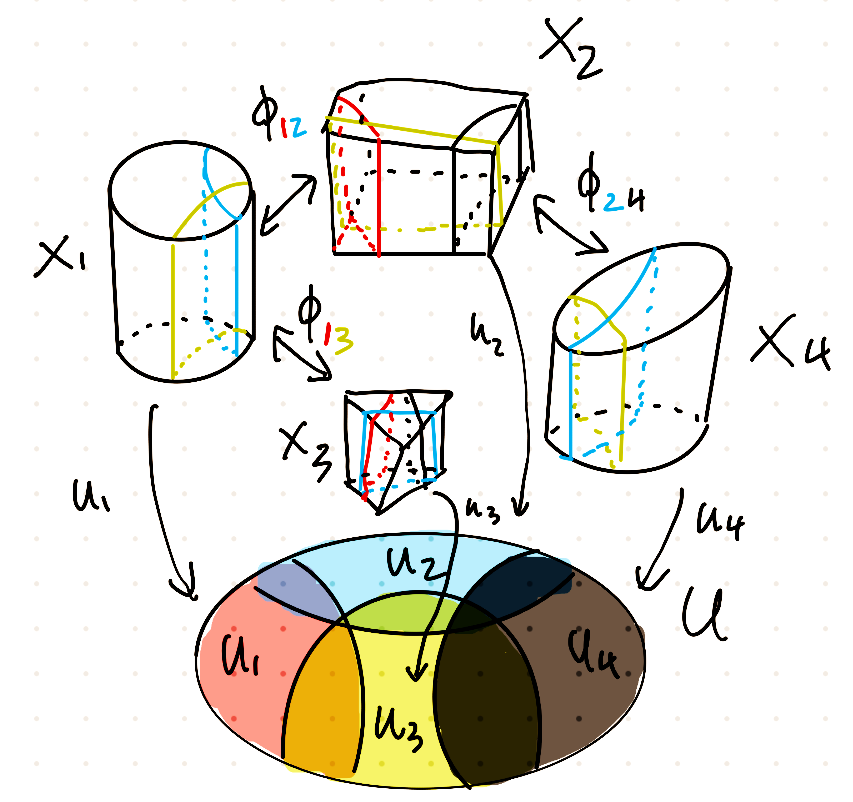
\includegraphics[width=11cm]{Images/Cocycle_condition.png}
\end{figure}
\end{remark}



\subsection{Descent data}

We are now ready to move onto stacks. The main idea is to generalize the type of \textit{local data} that we used to glue before.

For the rest of the chapter $\Cc$ is a site with a fixed Grothendieck topology and $\Fc$ is fibered category over $\Cc$.

\begin{definition}[]
Fix $U\in \Cc$ and a cover $\cpa{U_i\to U}\in \Cov(U)$. An \textbf{object with descent data} is a pair $(\cpa{\xi_i},\cpa{\phi_{ij}})$ where $\xi_i\in \Fc(U_i)$ for all $i$ and $\phi_{ij}:\pr_2^\ast\xi_j\to \pr_1^\ast\xi_i$ are isomorphisms which live in $\Fc(U_{ij})$ such that
\[\pr_{13}^\ast\phi_{ik}=\pr_{12}^\ast\phi_{ij}\circ \pr_{23}^\ast\phi_{jk}.\]
The $\phi_{ij}$ are called \textbf{transition isomorphisms}.
\end{definition}

If you are (very reasonably) getting confused with the pullbacks and indices, it may (or may not) be useful to admire \textit{the hypercube}
% https://q.uiver.app/#q=WzAsMTMsWzIsMSwiVV97amt9Il0sWzIsMywiVV97aWprfSJdLFsyLDQsIlVfaSJdLFsxLDQsIlVfe2lqfSJdLFszLDMsIlVfe2lrfSJdLFszLDEsIlVfayJdLFsxLDIsIlVfaiJdLFszLDUsIlxceGlfaSIsWzAsMTAwLDQ1LDFdXSxbMCw1LCJcXHByXzJeXFxhc3RcXHhpX2pcXHhyaWdodGFycm93e1xccGhpX3tpan19XFxwcl8xXlxcYXN0XFx4aV9pIixbMjM5LDEwMCw0MiwxXV0sWzAsMSwiXFx4aV9qIixbMCwxMDAsNDUsMV1dLFs0LDAsIlxceGlfayIsWzAsMTAwLDQ1LDFdXSxbMiwwLCJcXHByXzFee1xcYXN0fVxceGlfalxceGxlZnRhcnJvd3tcXHBoaV97amt9fVxccHJfMl5cXGFzdFxceGlfayIsWzIzOSwxMDAsNDIsMV1dLFs0LDMsIlxcYmVnaW57bWF0cml4fVxccHJfMl5cXGFzdFxceGlfa1xcXFxcXDtcXDtcXDtcXDtcXDtcXDtcXGRvd25hcnJvd3tcXHBoaV97aWt9fVxcXFxcXHByXzFeXFxhc3RcXHhpX2lcXGVuZHttYXRyaXh9IixbMjM5LDEwMCw0MiwxXV0sWzMsMiwiXFxwcl8xIl0sWzEsMywiXFxwcl97MTJ9IiwxXSxbMSw0LCJcXHByX3sxM30iLDFdLFs0LDIsIlxccHJfMSJdLFs0LDUsIlxccHJfMiIsMl0sWzEsMCwiXFxwcl97MjN9IiwxXSxbMCw1LCJcXHByXzIiXSxbMCw2LCJcXHByXzEiLDFdLFszLDYsIlxccHJfMiJdLFs3LDIsIiIsMSx7ImNvbG91ciI6WzAsMTAwLDQ1XSwic3R5bGUiOnsidGFpbCI6eyJuYW1lIjoibWFwcyB0byJ9fX1dLFs4LDksIiIsMCx7ImNvbG91ciI6WzIzOSwxMDAsNDJdfV0sWzksNiwiIiwxLHsiY29sb3VyIjpbMCwxMDAsNDVdLCJzdHlsZSI6eyJ0YWlsIjp7Im5hbWUiOiJtYXBzIHRvIn19fV0sWzgsMywiIiwxLHsib2Zmc2V0IjoyLCJjb2xvdXIiOlsyMzksMTAwLDQyXSwic3R5bGUiOnsidGFpbCI6eyJuYW1lIjoibWFwcyB0byJ9fX1dLFsxMCw1LCIiLDIseyJjb2xvdXIiOlswLDEwMCw0NV0sInN0eWxlIjp7InRhaWwiOnsibmFtZSI6Im1hcHMgdG8ifX19XSxbMTEsMCwiIiwyLHsib2Zmc2V0IjoyLCJjb2xvdXIiOlsyMzksMTAwLDQyXSwic3R5bGUiOnsidGFpbCI6eyJuYW1lIjoibWFwcyB0byJ9fX1dLFsxMSwxMCwiIiwwLHsiY29sb3VyIjpbMjM5LDEwMCw0Ml19XSxbMTIsNCwiIiwxLHsib2Zmc2V0IjoyLCJjb2xvdXIiOlsyMzksMTAwLDQyXSwic3R5bGUiOnsidGFpbCI6eyJuYW1lIjoibWFwcyB0byJ9fX1dLFsxMSw5LCIiLDAseyJjb2xvdXIiOlsyMzksMTAwLDQyXX1dLFs4LDcsIiIsMCx7ImNvbG91ciI6WzIzOSwxMDAsNDJdfV0sWzEyLDEwLCIiLDAseyJjb2xvdXIiOlsyMzksMTAwLDQyXX1dLFsxMiw3LCIiLDAseyJjb2xvdXIiOlsyMzksMTAwLDQyXX1dLFs4LDMsIiIsMSx7Im9mZnNldCI6LTIsImNvbG91ciI6WzIzOSwxMDAsNDJdLCJzdHlsZSI6eyJ0YWlsIjp7Im5hbWUiOiJtYXBzIHRvIn19fV0sWzEyLDQsIiIsMSx7Im9mZnNldCI6LTIsImNvbG91ciI6WzIzOSwxMDAsNDJdLCJzdHlsZSI6eyJ0YWlsIjp7Im5hbWUiOiJtYXBzIHRvIn19fV0sWzExLDAsIiIsMix7Im9mZnNldCI6LTIsImNvbG91ciI6WzIzOSwxMDAsNDJdLCJzdHlsZSI6eyJ0YWlsIjp7Im5hbWUiOiJtYXBzIHRvIn19fV1d
\[\begin{tikzcd}
	&& \textcolor{rgb,255:red,0;green,4;blue,214}{{\pr_1^{\ast}\xi_j\xleftarrow{\phi_{jk}}\pr_2^\ast\xi_k}} && \textcolor{rgb,255:red,230;green,0;blue,0}{{\xi_k}} \\
	\textcolor{rgb,255:red,230;green,0;blue,0}{{\xi_j}} && {U_{jk}} & {U_k} \\
	& {U_j} \\
	&& {U_{ijk}} & {U_{ik}} & \textcolor{rgb,255:red,0;green,4;blue,214}{\begin{array}{c} \begin{matrix}\pr_2^\ast\xi_k\\\;\;\;\;\;\;\downarrow{\phi_{ik}}\\\pr_1^\ast\xi_i\end{matrix} \end{array}} \\
	& {U_{ij}} & {U_i} \\
	\textcolor{rgb,255:red,0;green,4;blue,214}{{\pr_2^\ast\xi_j\xrightarrow{\phi_{ij}}\pr_1^\ast\xi_i}} &&& \textcolor{rgb,255:red,230;green,0;blue,0}{{\xi_i}}
	\arrow[color={rgb,255:red,0;green,4;blue,214}, from=1-3, to=1-5]
	\arrow[color={rgb,255:red,0;green,4;blue,214}, from=1-3, to=2-1]
	\arrow[shift right=2, color={rgb,255:red,0;green,4;blue,214}, maps to, from=1-3, to=2-3]
	\arrow[shift left=2, color={rgb,255:red,0;green,4;blue,214}, maps to, from=1-3, to=2-3]
	\arrow[color={rgb,255:red,230;green,0;blue,0}, maps to, from=1-5, to=2-4]
	\arrow[color={rgb,255:red,230;green,0;blue,0}, maps to, from=2-1, to=3-2]
	\arrow["{\pr_2}", from=2-3, to=2-4]
	\arrow["{\pr_1}"{description}, from=2-3, to=3-2]
	\arrow["{\pr_{23}}"{description}, from=4-3, to=2-3]
	\arrow["{\pr_{13}}"{description}, from=4-3, to=4-4]
	\arrow["{\pr_{12}}"{description}, from=4-3, to=5-2]
	\arrow["{\pr_2}"', from=4-4, to=2-4]
	\arrow["{\pr_1}", from=4-4, to=5-3]
	\arrow[color={rgb,255:red,0;green,4;blue,214}, from=4-5, to=1-5]
	\arrow[shift right=2, color={rgb,255:red,0;green,4;blue,214}, maps to, from=4-5, to=4-4]
	\arrow[shift left=2, color={rgb,255:red,0;green,4;blue,214}, maps to, from=4-5, to=4-4]
	\arrow[color={rgb,255:red,0;green,4;blue,214}, from=4-5, to=6-4]
	\arrow["{\pr_2}", from=5-2, to=3-2]
	\arrow["{\pr_1}", from=5-2, to=5-3]
	\arrow[color={rgb,255:red,0;green,4;blue,214}, from=6-1, to=2-1]
	\arrow[shift right=2, color={rgb,255:red,0;green,4;blue,214}, maps to, from=6-1, to=5-2]
	\arrow[shift left=2, color={rgb,255:red,0;green,4;blue,214}, maps to, from=6-1, to=5-2]
	\arrow[color={rgb,255:red,0;green,4;blue,214}, from=6-1, to=6-4]
	\arrow[color={rgb,255:red,230;green,0;blue,0}, maps to, from=6-4, to=5-3]
\end{tikzcd}\]



\begin{notation}[]
Let $\Cc$ be a site, $\Fc$ fibered over $\Cc$, $U\in \Cc$ and $\cpa{U_i\to U}\in \Cov(U)$. Objects with descent data over $\cpa{U_i\to U}$ form a category\footnote{the morphisms are collections of maps and commutative diagrams which are compatible with the indices.}, which we denote using 
\[\Fc(\cpa{U_i\to U}).\]
\end{notation}


\begin{remark}
Fix $U\in \Cc$, $\cpa{u_i:U_i\to U}\in \Cov(U)$ and $\xi\in \Fc(U)$. From $\xi$ we can obtain an object with descent data by restriction. To be more precise, we can define
\[\xi_i=u_i^\ast\xi,\qquad \phi_{ij}:\pr_2^\ast u_j^\ast\xi\to \pr_1^\ast u_i^\ast \xi\]
where $\phi_{ij}$ is the canonical isomorphism induced by the fact that both objects amount to the pullback of $\xi$ along $U_{ij}\to U$. The resulting object with descent data is $(\cpa{\xi_i},\cpa{\phi_{ij}})$.
\end{remark}

\begin{center}
\textit{What we have described is actually a functor from $\Fc(U)$ to $\Fc(\cpa{U_i\to U})$.}
\end{center}

\begin{definition}[]
An object with descent data is called \textbf{effective} if it is in the essential image of the functor above.
\end{definition}

\noindent We are now finally ready to define prestacks and stacks:
\begin{definition}[]
Let $\Fc$ be a fibered category over $\Cc$ site. $\Fc$ is a
\begin{itemize}
	\item \textbf{prestack} if for all $U\in \Cc$ and all $\cpa{U_i\to U}\in \Cov(U)$, the functor
	\[\Fc(U)\to \Fc(\cpa{U_i\to U})\]
	is \textit{fully faithful}.
	\item \textbf{stack} if for all $U\in \Cc$ and all $\cpa{U_i\to U}\in \Cov(U)$, the functor
	\[\Fc(U)\to \Fc(\cpa{U_i\to U})\]
	is an \textit{equivalence}.
\end{itemize}
\end{definition}

\begin{remark}
The two conditions can be intuitively understood as:
\begin{itemize}
\item A prestack is a fibered category where if two objects are the same locally (taking into account gluing) then they are isomorphic.
\item A stack is a prestack where all descent data glues to an object.
\end{itemize}
\end{remark}

Another way in which we can intepret the prestack condition is given in the following

\begin{proposition}
Let $\Fc$ be fibered over $\Cc$ site. $\Fc$ is a prestack if and only if for all $U\in \Cc$ and all $\xi,\eta\in \Fc(U)$, the functor
\[\ul{\Hom}_U(\xi,\eta):\funcDef{(\Cc/U)\op}{\Set}{f:Z\to U}{\Hom_Z(f^\ast\xi,f^\ast \eta)}\]
is a sheaf on $\Cc/U$.
\end{proposition}
\begin{proof}[Sketch]
Fix $U\in \Cc$ and $\cpa{U_i\to U}\in \Cov(U)$. The functor $\Fc(U)\to \Fc(\cpa{U_i\to U})$ being fully faithful means that for all $\xi,\eta\in \Fc(U)$ we have
\[\Hom_U(\xi,\eta)\cong \Hom_{\cpa{U_i\to U}}((\cpa{\xi_i},\cpa{\al_{ij}}),(\cpa{\eta_i},\cpa{\beta_{ij}}))\]
where $(\cpa{\xi_i},\cpa{\al_{ij}})$ is the image of $\xi$ and similarly for the other object and $\eta$.

Concretely, this means that maps $\xi\to \eta$ can be defined uniquely on an open cover, which is exactly what it means for $\ul{\Hom}_U(\xi,\eta)$ to be a sheaf.
\end{proof}

\begin{corollary}
$\Arr(\Top)$ is a stack.
\end{corollary}

We close the chapter by noting that when $\Fc/\Cc$ is fibered in sets, we find the notions of separated presheaf and sheaf over $\Cc$ respectively, meaning that we have, in some very precise sense, defined \textit{sheaves in categories}. This concept will be trated in more detail in the next chapter.
\begin{proposition}
Let $\Cc$ be a site and consider a functor $F:\Cc\op\to \Set$. Identify $F$ with the fibered category it defines. Then
\begin{itemize}
	\item $F$ is a prestack if and only if it is a separated presheaf,
	\item $F$ is a stack if and only if $F$ is a sheaf.
\end{itemize}
\end{proposition}

\begin{example}
The fibered category associated to an object $X\in \Cc$ is a stack because it corresponds to the functor $h_X=\Hom_\Cc(\cdot, X)$.
\end{example}



\chapter{Algebraic Stacks}
\begin{center}
	{\huge Speaker: Pietro Leonardini}
\end{center}
\bigskip

\section{Motivation: moduli problems}
\subsection{The dream}
Let us recall what an elliptic curve is:
\begin{definition}[Elliptic curve]
An \textbf{elliptic curve} over $k$ is a 1-dimensional scheme $C\to \Spec k$ over $k$ which is geometrically integral, proper, smooth and of genus\footnote{the genus is $\dim_k H^1(C,\Oc_C)$} 1 with a fixed $k$-rational point $e:\Spec k\to C$.
\end{definition}

Since the relative approach is central in the theory of schemes, we may want to define an elliptic curve over some base scheme $S$. The most sensible approach is to say that an elliptic curve over $S$ should be a ``family of elliptic curves parametrized by $S$". Formally:

\begin{definition}[Elliptic curve over $S$]
An \textbf{elliptic curve} over $S$ is a proper, smooth, flat morphism of schemes $p:E\to S$ with a fixed section $e:S\to E$ of $p$ such that for all $\Spec \Omega$ geometric point, the pullback is an elliptic curve over $\Omega$:
% https://q.uiver.app/#q=WzAsNCxbMSwwLCJFIl0sWzEsMSwiUyJdLFswLDEsIlxcU3BlYyBcXE9tZWdhIl0sWzAsMCwiRVxcdGltZXNfU1xcU3BlY1xcT21lZ2EgIl0sWzMsMF0sWzMsMl0sWzIsMV0sWzAsMV1d
\[\begin{tikzcd}
	{E\times_S\Spec\Omega } & E \\
	{\Spec \Omega} & S
	\arrow[from=1-1, to=1-2]
	\arrow[from=1-1, to=2-1]
	\arrow[from=1-2, to=2-2]
	\arrow[from=2-1, to=2-2]
\end{tikzcd}\]
\end{definition}

When studying elliptic curves it would be useful to find some space $M_{1,1}$ such that for every family $E\to S$ we have a unique $\phi:S\to M_{1,1}$ such that
% https://q.uiver.app/#q=WzAsNCxbMCwwLCJFIl0sWzAsMSwiUyJdLFsxLDEsIk1fezEsMX0iXSxbMSwwLCJcXEVjIl0sWzAsMV0sWzMsMl0sWzAsM10sWzEsMiwiXFxwaGkiLDJdXQ==
\[\begin{tikzcd}
	E & \Ec \\
	S & {M_{1,1}}
	\arrow[from=1-1, to=1-2]
	\arrow[from=1-1, to=2-1]
	\arrow[from=1-2, to=2-2]
	\arrow["\phi"', from=2-1, to=2-2]
\end{tikzcd}\]
that is, we would be very happy if all families of elliptic curves could be described as the pullback of some \textit{universal family} $\Ec$ over $M_{1,1}$ along some morphism $S\to M_{1,1}$. Intuitively, the universal family should be the one defined by the fact that the fiber over a point of $M_{1,1}$ is the elliptic curve corresponding to that point. The morphism should be the one that to each point of $S$ assigns some elliptic curve, i.e. a point of $M_{1,1}$ (of course this naive view is too simple when dealing with schemes but it motivates why we look for such a map).
\bigskip

A useful way to formulate this problem is to define the following functor\footnote{we technically have no guarantee that families over a scheme should form a set. This issue will be solved automatically later when we consider a fibered category over $\Sch$ instead of a functor.}
\[F:\functorDef{\Sch\op}{\Set}{S}{\cpa{E\to S\mid \text{elliptic curves}}/\text{iso.}}{f:T\to S}{(E_1\to S)\mapsto (f^\ast E_1\to T)}\]
We can re-formulate the requirements on $M_{1,1}$ by saying that $M_{1,1}$ should \textbf{represent} this functor, i.e. there is a natural isomorphism of functors
\[h_{M_{1,1}}\cong F\]
where $h_{M_{1,1}}$ is the contravariant $\Hom$-functor associated to $M_{1,1}$.
\medskip

We recall the following simple but foundational result
\begin{theorem}[Yoneda lemma]
There is a natural correspondence
\[\Hom(h_X,F)\leftrightarrow F(X)\]
\end{theorem}
\begin{proof}[sketch]
Suppose we have a natural transformation $\phi:h_X\to F$, then we can find an element of $F(X)$ by taking $\phi_X(id_X)=\xi$.

Let us now fix an element $\xi\in F(X)$. Let $T$ be a scheme. We may construct a map $\Hom(T,X)\to F(T)$ by sending $f:T\to X$ to $F(f)(\xi)$. If $g:T\to S$ is a morphism then $\eta:f\mapsto g\circ f$ is mapped to $F(g):F(S)\to F(T)$. It is easy to check that this defines a natural transformation $h_X\to F$ and that the two constructions are inverses of each other.
\end{proof}
\begin{corollary}
The functor $\Cc\to \Fun(\Cc\op,\Set)$ that sends $X$ to $h_X$ is fully faithful.
\end{corollary}


\subsection{A good attempt}
Let us try to find some way of parametrizing isomorphism classes of elliptic curves. The main idea comes from the following fact:

\begin{fact}
If $\cha k\neq2,3$ then every elliptic curve is isomorphic over $\ol k$ to some
\[E_\la:y^2=x(x-1)(x-\la)\] 
for some $\la\in k\bs\cpa{0,1}$.
\end{fact}

\begin{definition}[$j$-invariant]
Let
\[j(E_\la)=2^8\frac{(\la^2-\la+1)^3}{\la^2(\la-1)^2}\]
\end{definition}

\begin{fact}
The map
\[\phi:\funcDef{\ol k\bs\cpa{0,1}}{\ol k}{\la}{j(E_\la)}\]
is surjective and $6:1$ except in $j=0$ and $j=1728$, where it is $2:1$ and $3:1$ respectively.
\end{fact}

\begin{fact}
Two elliptic curves are isomorphic over $\ol k$ if and only if they have the same $j$-invariant.
\end{fact}


\begin{theorem}
Let $E\to S$ be an elliptic curve, then there exists a Zariski affine open over of $S$ given by $\cpa{U_i=\Spec A_i}$ such that for all $i$
% https://q.uiver.app/#q=WzAsNCxbMCwwLCJFX2k6PVxcU3BlY1xccGF7XFxkZnJhY3tBX2lbeCx5XX17KHleMi14XjMtQXgtQil9fSJdLFswLDEsIlxcU3BlYyBBX2kiXSxbMSwxLCJTIl0sWzEsMCwiRSJdLFswLDFdLFszLDJdLFswLDNdLFsxLDJdXQ==
\[\begin{tikzcd}
	{E_i:=\Spec\pa{\dfrac{A_i[x,y]}{(y^2-x^3-Ax-B)}}} & E \\
	{\Spec A_i} & S
	\arrow[from=1-1, to=1-2]
	\arrow[from=1-1, to=2-1]
	\arrow[from=1-2, to=2-2]
	\arrow[from=2-1, to=2-2]
\end{tikzcd}\]
for some $A,B\in A_i$.
\end{theorem}

\begin{remark}
With $E\to S$ elliptic curve and a cover like above, the $j$-invariants of $E_i\to \Spec A_i$ are sections of the structure sheaf of $\Spec A_i$ which coincide on the intersection, so they glue to a section $j\in \Gamma(S,\Oc_S)$.
\end{remark}

\noindent
From this discussion it follows that the best candidate for $M_{1,1}$ is $\A^1$ where the curve over $j\in \A^1$ is the one with that $j$-invariant.
Unfortunately $\A^1$ does not work.

\begin{example}
Suppose $\A^1$ represents the functor $F$ from before. Consider then the two families
% https://q.uiver.app/#q=WzAsNCxbMCwwLCJcXFNwZWNcXHBhe1xcZnJhY3trW3gseSx0XlxccG1dfXsoeV4yLXheMyt0KX19Il0sWzAsMSwiXFxTcGVjIGtbdCx0XFxpaV0iXSxbMSwxLCJcXEFeMSJdLFsxLDAsIlxceGkiXSxbMCwxXSxbMywyXSxbMCwzXSxbMSwyXV0=
\[\begin{tikzcd}
	{\Spec\pa{\frac{k[x,y,t^\pm]}{(y^2-x^3+t)}}} & \xi \\
	{\Spec k[t,t\ii]} & {\A^1}
	\arrow[from=1-1, to=1-2]
	\arrow[from=1-1, to=2-1]
	\arrow[from=1-2, to=2-2]
	\arrow[from=2-1, to=2-2]
\end{tikzcd}\]
and
% https://q.uiver.app/#q=WzAsNSxbMCwxLCJcXFNwZWNcXHBhe1xcZnJhY3trW3gseSx0XlxccG1dfXsoeV4yLXheMysxKX19Il0sWzAsMiwiXFxTcGVjIGtbdCx0XFxpaV0iXSxbMSwyLCJcXEFeMSJdLFsxLDEsIlxceGkiXSxbMCwwLCJcXFNwZWNcXHBhe1xcZnJhY3trW3gseV19eyh5XjIteF4zKzEpfX1cXHRpbWVzXFxTcGVjXFxwYXtrW3Ree1xccG0xfV19Il0sWzAsMV0sWzMsMl0sWzAsM10sWzEsMl0sWzQsMCwiPSIsMSx7InN0eWxlIjp7ImJvZHkiOnsibmFtZSI6Im5vbmUifSwiaGVhZCI6eyJuYW1lIjoibm9uZSJ9fX1dXQ==
\[\begin{tikzcd}
	{\Spec\pa{\frac{k[x,y]}{(y^2-x^3+1)}}\times\Spec\pa{k[t^{\pm1}]}} \\
	{\Spec\pa{\frac{k[x,y,t^\pm]}{(y^2-x^3+1)}}} & \xi \\
	{\Spec k[t,t\ii]} & {\A^1}
	\arrow["{=}"{description}, draw=none, from=1-1, to=2-1]
	\arrow[from=2-1, to=2-2]
	\arrow[from=2-1, to=3-1]
	\arrow[from=2-2, to=3-2]
	\arrow[from=3-1, to=3-2]
\end{tikzcd}\]
If $\A^1$ represented the functor, these two families should be isomorphic (both are pullbacks along $\Spec k[t,t\ii]\to \A^1$ of the universal family), but they are not:

it is possible to prove via the $j$-invariants that two Weierstrass equations yield isomorphic curves if and only if there exists some $u\in k[t^{\pm1}]$ such that substituting $x$ with $u^2x$ and $y$ with $u^3y$ transforms one equation into the other up to factoring out powers of $u$. Therefore we require for there to exist some $u$ such that
\[u^6y^2-u^6x^3+t=u^k(y^2-x^3+1)\coimplies t=u^6\]
and this is impossible.
\end{example}

\begin{remark}
A slogan to keep in mind is
\begin{center}
    \textit{The presence of non-trivial automorphisms prevent the moduli problem from having a fine moduli space.}
\end{center}
\end{remark}

\begin{example}
If we consider the same families from before but now over the base $\Spec\frac{k[t^{\pm1},w]}{(t-w^6)}$ instead of $\Spec k[t^{\pm 1}]$, they now become isomorphic, that is
\[\frac{k[x,y,t^\pm,w]}{(y^2-x^3+1,w^6-t)}\cong \frac{k[x,y,t^\pm,w]}{(y^2-x^3+t,w^6-t)}.\]
This is because now we can choose $u=w$ with the notation from before. 

The idea behind this observation is that if we allow ourselves to look at finer topologies on $\Sch$ we may be able to solve our representability issue. We are starting to see how viewing $F$ as a functor is not enough; we should view it as some kind of sheaf.
\end{example}


\subsection{Our dreams crumble?}

So, what now? We have two options:
\begin{itemize}
    \item Rigidify the problem (GIT approach)
    \item Enlarge the category among which we search for the moduli space (Stacky approach) 
\end{itemize}

\begin{notation}
From now on we identify the scheme $X$ with the functor $h_X:\Sch\op\to \Set$ and we identify it with the appropriate fibered category over $\Sch$. 
\end{notation}
\begin{remark}
$X(k)=\Hom(\Spec k,X)$.
\end{remark}

\begin{center}
	{\Large The main idea:}
\end{center}
Instead of the functor $F$ from before \textbf{we consider the category} $\Mc_{1,1}$ \textbf{fibered in groupoids} over $\Sch$ defined the same way.

\begin{remark}
The issue with families forming sets is now irrelevant. To be more precise, the groupoid associated to a scheme $S$ is the one whose objects are elliptic curves over $S$ and whose morphisms are isomorphisms of families (making this category a groupoid by construction).
\end{remark}


\begin{theorem}
The fibered category $\Mc_{1,1}$ is a stack for the fpqc topology.
\end{theorem}
\begin{proof}
Olsson \cite{olsson2016algebraic}, chapter 13
\end{proof}

\begin{remark}
A morphism $\phi :X\to\Mc_{1,1}$ of stacks corresponds by (a version of) the Yoneda lemma to an element of the fiber $\Mc_{1,1}(X)$.
\bigskip

\noindent Said another way, there is a correspondence between families of curves over $X$ (the category $\Mc_{1,1}(X)$) and morphisms $X\to \Mc_{1,1}$.
\end{remark}

From a categorical point of view, $\Mc_{1,1}$ does exactly what we want. Now we try to understand in which ways it can be thought of as a space.


\section{Algebraic stacks}
If we want to think about stacks in a geometric way, we may want to impose some ``good behaviour" conditions. For example, one thing we may require is that if two ``normal" objects (for example schemes) live inside our stack, their intersection should still be a ``normal" object. The key definition to formalize this idea is
\begin{definition}[Representable morphism]
Let $\Xc\to \Yc$ be a morphism of stacks, then it is said to be \textbf{representable} if for all schemes $T$ and morphisms $T\to \Yc$ there exists an algebraic space $V$ such that
% https://q.uiver.app/#q=WzAsNCxbMCwwLCJWIl0sWzAsMSwiXFxYYyJdLFsxLDEsIlxcWWMiXSxbMSwwLCJUIl0sWzAsMV0sWzMsMl0sWzAsM10sWzEsMl1d
\[\begin{tikzcd}
	V & T \\
	\Xc & \Yc
	\arrow[from=1-1, to=1-2]
	\arrow[from=1-1, to=2-1]
	\arrow[from=1-2, to=2-2]
	\arrow[from=2-1, to=2-2]
\end{tikzcd}\]
is cartesian.

We say that a morphism of stacks $\Xc\to \Yc$ has a property $\Pc$ for $\Pc$ a property of morphisms of schemes/algebraic spaces which is stable under base change if the morphism is representable and for all $T\to\Yc$, the induced arrow $V\to T$ as above has the property $\Pc$.
\end{definition}

\begin{remark}
The properties ``begin smooth", ``begin surjective" and ``begin \'etale" are stable under base change.
\end{remark}

\begin{definition}[Algebraic stack]
A stack over a scheme $S$, i.e. a morphism of stacks $\Xc\to S$ is said to be \textbf{algebraic} if
\begin{enumerate}
\item the diagonal $\Delta:\Xc\to \Xc\times_S\Xc$ is representable and 
\item there exists a smooth and surjective morphism $\pi:X\to \Xc$ for $X$ scheme. This scheme is called an \textbf{atlas} for the algebraic stack.
\end{enumerate}
If $\pi:X\to \Xc$ is \'etale then $\Xc\to S$ is called a \textbf{Deligne-Mumford stack}.
\end{definition}

\begin{remark}
Property 1. looks very mysterious but the following is an equivalent and, perhaps clearer, formulation: for all $T,U$ schemes, the fibered product $T\times_\Xc U$ exists and is an algebraic space. We may think of this as saying that ``intersecting schemes in a stack gives an algebraic space".

Thinking about this set-theoretically may help in understanding the equivalence.
\end{remark}

\begin{remark}
Property 2. can be thought of as ``finiteness" condition. The case of Deligne-Mumford stacks makes this even clearer because \'etale morphisms can be thought of as unramified covers, so we are saying that our stack admits a cover with total space being a scheme.
\end{remark}






\section{Quotient stacks}

Let us study a specific type of algebraic stacks: quotients.

\begin{definition}[$G$-fibration]
Let $X$ be a scheme, $G$ a group scheme. A \textbf{$G$-fibration} over $X$ is a scheme $\xi$ with an action $\mu:G\times \xi\to \xi$ and a $G$-invariant morphism $\pi:\xi\to X$, that is, we have a commutative diagram
% https://q.uiver.app/#q=WzAsNCxbMCwwLCJHXFx0aW1lcyBcXHhpIl0sWzAsMSwiXFx4aSJdLFsxLDAsIlxceGkiXSxbMSwxLCJYIl0sWzAsMiwiXFxtdSJdLFswLDEsIlxccGlfMiIsMl0sWzIsMywiXFxwaSJdLFsxLDMsIlxccGkiLDJdXQ==
\[\begin{tikzcd}
	{G\times \xi} & \xi \\
	\xi & X
	\arrow["\mu", from=1-1, to=1-2]
	\arrow["{\pi_2}"', from=1-1, to=2-1]
	\arrow["\pi", from=1-2, to=2-2]
	\arrow["\pi"', from=2-1, to=2-2]
\end{tikzcd}\]
\end{definition}

\begin{example}
$\xi=G\times X$ with the obvious projection $\xi\to X$ is a $G$-fibration. This is called the \textbf{trivial} $G$-fibration.
\end{example}

\begin{definition}[Principal $G$-bundle]
A \textbf{principal $G$-bundle} with respect to the fpqc (or fppf, \'etale etc) topology is a $G$-fibration which is locally trivial, i.e. there exists a cover $\cpa{U_i\to X}$ such that $\xi\res {U_i}\to U_i$ is isomorphic to $G\times U_i\to U_i$.
\end{definition}


\begin{proposition}
Let $X$ be a scheme and $G$ a linear algebraic group acting on $X$ via $\mu:X\times G\to X$. Assume that the action is free\footnote{for all schemes $\mu_T:X(T)\times G(T)\to X(T)$ is a free action of $G(T)$}, then $X/G$ exists as an algebraic space.

Moreover $\rho:X\to X/G$ is a principal $G$-bundle with respect to the \'etale topology and the following is cartesian
% https://q.uiver.app/#q=WzAsNCxbMCwwLCJYXFx0aW1lcyBHIl0sWzAsMSwiWCJdLFsxLDEsIlgvRyJdLFsxLDAsIlgiXSxbMCwxLCJcXG11IiwyXSxbMywyLCJcXHJobyJdLFswLDMsIlxccGlfMSJdLFsxLDJdXQ==
\[\begin{tikzcd}
	{X\times G} & X \\
	X & {X/G}
	\arrow["{\pi_1}", from=1-1, to=1-2]
	\arrow["\mu"', from=1-1, to=2-1]
	\arrow["\rho", from=1-2, to=2-2]
	\arrow[from=2-1, to=2-2]
\end{tikzcd}\]
\end{proposition}

\begin{remark}
If we fix $f:U\to X/G$ and take $\xi$ to be the pullback of $X\to X/G$ along $U\to X/G$ 
% https://q.uiver.app/#q=WzAsNCxbMCwwLCJcXHhpIl0sWzAsMSwiVSJdLFsxLDAsIlgiXSxbMSwxLCJYL0ciXSxbMCwyLCJcXGFsIl0sWzAsMSwiXFxwaSIsMl0sWzIsMywiXFxyaG8iXSxbMSwzLCJmIiwyXV0=
\[\begin{tikzcd}
	\xi & X \\
	U & {X/G}
	\arrow["\al", from=1-1, to=1-2]
	\arrow["\pi"', from=1-1, to=2-1]
	\arrow["\rho", from=1-2, to=2-2]
	\arrow["f"', from=2-1, to=2-2]
\end{tikzcd}\]
then
\begin{enumerate}
    \item $\pi:\xi\to U$ is a $G$-bundle and
    \item $\al:\xi\to X$ is $G$-equivariant.
\end{enumerate}
\end{remark}


\begin{definition}[]
Let $X$ be a scheme and $G$ a smooth linear algebraic group acting on $X$, the \textbf{quotient stack} $[X/G]$ is the fibered category over schemes
\[U\mapsto \cpa{(\pi:\xi\to U, \al:\xi\to X)\mid \pi\text{ principal $G$-bundle, $\al$ $G$-equivariant}}/\sim\]
If $X=\Spec k$, $[\Spec k/G]=\B G$ is called the \textbf{classifying space} of $G$.
\end{definition}



\begin{theorem}
    $[X/G]$ is an algebraic stack
\end{theorem}

Let us quickly convince ourselves that $[X/G]$ should be an algebraic stack by looking at what the atlas should be:
\setlength{\leftmargini}{0cm}
\begin{itemize}
\item[] The obvious candidate for an atlas is $\pi:X\to [X/G]$ (think ``quotient map is a cover"). This morphism corresponds via the Yoneda lemma to a family of principal $G$-bundles over $X$, which is
% https://q.uiver.app/#q=WzAsMyxbMCwwLCJYXFx0aW1lcyBHIl0sWzAsMSwiWCJdLFsxLDAsIlgiXSxbMCwxLCJcXG11IiwyXSxbMCwyLCJcXHBpXzEiXV0=
\[\begin{tikzcd}
	{X\times G} & X \\
	X
	\arrow["{\pi_1}", from=1-1, to=1-2]
	\arrow["\mu"', from=1-1, to=2-1]
\end{tikzcd}\]
\item[] If we fix $\vp:U\to [X/G]$, this corresponds to a family
% https://q.uiver.app/#q=WzAsMyxbMCwwLCJcXHhpIl0sWzAsMSwiVSJdLFsxLDAsIlgiXSxbMCwxLCJcXGV0YSIsMl0sWzAsMiwiXFxhbCJdXQ==
\[\begin{tikzcd}
	\xi & X \\
	U
	\arrow["\al", from=1-1, to=1-2]
	\arrow["\eta"', from=1-1, to=2-1]
\end{tikzcd}\]
with $\eta:\xi\to U$ smooth and surjective (not obvious but provable)
\end{itemize}
\setlength{\leftmargini}{0.5cm} 





\subsection{Back to elliptic curves}
Let us consider the scheme\footnote{$U\subseteq\A^2$ is the possible pairs $(A,B)$ of coefficients in a Weierstrass form for an elliptic curve. Localizing at the discriminant enforces that for any point $(A,B)\in U$, the curve $y^2=x^3+Ax+B$ is an elliptic curve.} $U=\Spec k[A,B,1/\Delta]$ where $\Delta=-16(4A^3+27B^2)$, and let $G=\G_m=k[u^{\pm 1}]$.
$G$ actis on $U$ by looking at equivalent Weierstrass forms via the change of variables
\[x\mapsto u^2 x, y\mapsto u^3 y.\]
Concretely, the action maps $A$ to $u^{-4}A$, $B$ to $u^{-6}B$ and $\Delta$ to $u^{-12}\Delta$.

\begin{fact}
$\Mc_{1,1}\cong [U/G]$.
\end{fact}









\part{Intersection theory}
\chapter{Definition of Chow ring}
\begin{center}
	{\huge Speaker: Andrea Gallese}
\end{center}
\bigskip

\noindent
The main reference for this chapter is \cite{eisenbud20163264}.

\section{Algebrizing intersection}
Think back to our roots: algebraic geometry is the study of solutions to systems of polynomial equations, which we can think of as intersecting some geometric objects. It seems reasonable then that we ought to study carefully what it means for varieties to intersect. 

One way we may approach this question can we make intersection into an algebraic operation? The answer is yes and the algebraic objects which come out from this idea are the Chow rings.

\bigskip

\noindent
In this chapter we take $k$ to be an alegbraically closed field. All schemes will be smooth and of finite type\footnote{note that this implies noetherian} over $k$.

\subsection{Chow group}
\begin{definition}[]
Let $X$ be a scheme as above. We define its \textbf{algebraic cycles} to be
\[Z(X)=\Z\spa{\text{integral closed subschemes of $X$}}=\bigoplus_{k}Z_k(X).\]
where $Z_k(X)$ is the same thing for subschemes of dimension $k$.
\end{definition}

\begin{remark}
$Z(X)=Z(X^{red})$.
\end{remark}

\begin{remark}
We may also grade $Z(X)$ with respect to codimension instead of dimension, which we will do eventually.
\end{remark}


\begin{definition}
Given $Y\subseteq X$ closed subscheme with irreducible components $Y_1,\cdots, Y_r$, we define the \textbf{algebraic cycle associated to $Y$} to be
\[\ps{Y}=\sum_{i=1}^r \ell_i[Y_i]\]
where\footnote{length of the module over itself. In particular, if $\Oc_{Y,y_i}$ is reduced then $\ell_i=1$.} $\ell_i=\length(\Oc_{Y,y_i})$ for $y_i\in Y_i$ the generic point.
\end{definition}

\begin{example}
Consider $V(xy)\subseteq \A^2$. The irreducible components are $V(x)$ and $V(y)$ with generic points $(x)$ and $(y)$ respectively. Note that $\pa{\frac{k[x,y]}{(x)}}_{(x)}=k(y)$, so it is reduced and the length is 1, same idea for the other irreducible component.
\medskip

Consider now $V(x^2)\subseteq \A^2$. The only irreducible component is $V(x)$ with generic point $(x)$ but now $\pa{\frac{k[x,y]}{(x^2)}}_{(x)}$ is not reduced because $x\neq 0$ and $x^2=0$. This is reflected in the fact that this ring has length 2, which can be seen by noting that
\[(0)\subsetneq (x)\subsetneq (1)\]
is a composition series. The fact that the length is 2 recovers the fact that we started with $V(x^2)$ instead of $V(x)$.
\end{example}

The group of cycles is way too large for any practical purpose, so we want to define when two cycles should be thought of as the same. We give the following definition in hope that it models ``continuous deformations" in some sense:

\begin{definition}[]
We define the subgroup $\Rat(X)$ of $Z(X)$ to be the one which is generated as follows
\[\Rat(X)=\ps{\ps{\Phi\cap (\cpa{t_0}\times X)}-\ps{\Phi\cap (\cpa{t_1}\times X)}}\]
where $Z$ varies among integral subvarieties of $X\times \Pj^1$ and $t_0,t_1$ are rational points of the projective line, i.e. $t_0,t_1\in \Pj^1(k)$.
\end{definition}

We can now define our main character

\begin{definition}[]
Let $X$ be a smooth scheme of finite type over $k$. We define its \textbf{Chow group} as the quotient
\[CH(X)=\frac{Z(X)}{\Rat(X)}.\]
If two cycles give the same element in $CH(X)$ we say that they are \textbf{rationally equivalent} and we may write this with $\sim$.
\end{definition}

\begin{remark}
The Chow group is graded by dimension and by codimension.
\end{remark}

\begin{example}
The cycles $[y=0]+[x=0]$ and $[xy=1]$ in $\A^2$ are rationally equivalent. Consider 
\[\Phi=V(xy-t)\subseteq \Pj^1\times \A^2\]
where $t$ is the coordinate\footnote{to be more precise, if the coordinates are $[s:t]$ we are taking $\Phi=V(sxy-t)$} of $\Pj^1$. Let $t_0=0$ and $t_1=1$, which are clearly rational points of $\Pj^1$, then we have
\[[y=0]+[x=0]=\ps{V(xy)}=\ps{\Phi\cap \cpa{0}\times \A^2}\]
and similarly for the other cycle. Thus $[y=0]+[x=0]\sim [xy=1]$.
\begin{figure}[!htb]
	\centering
	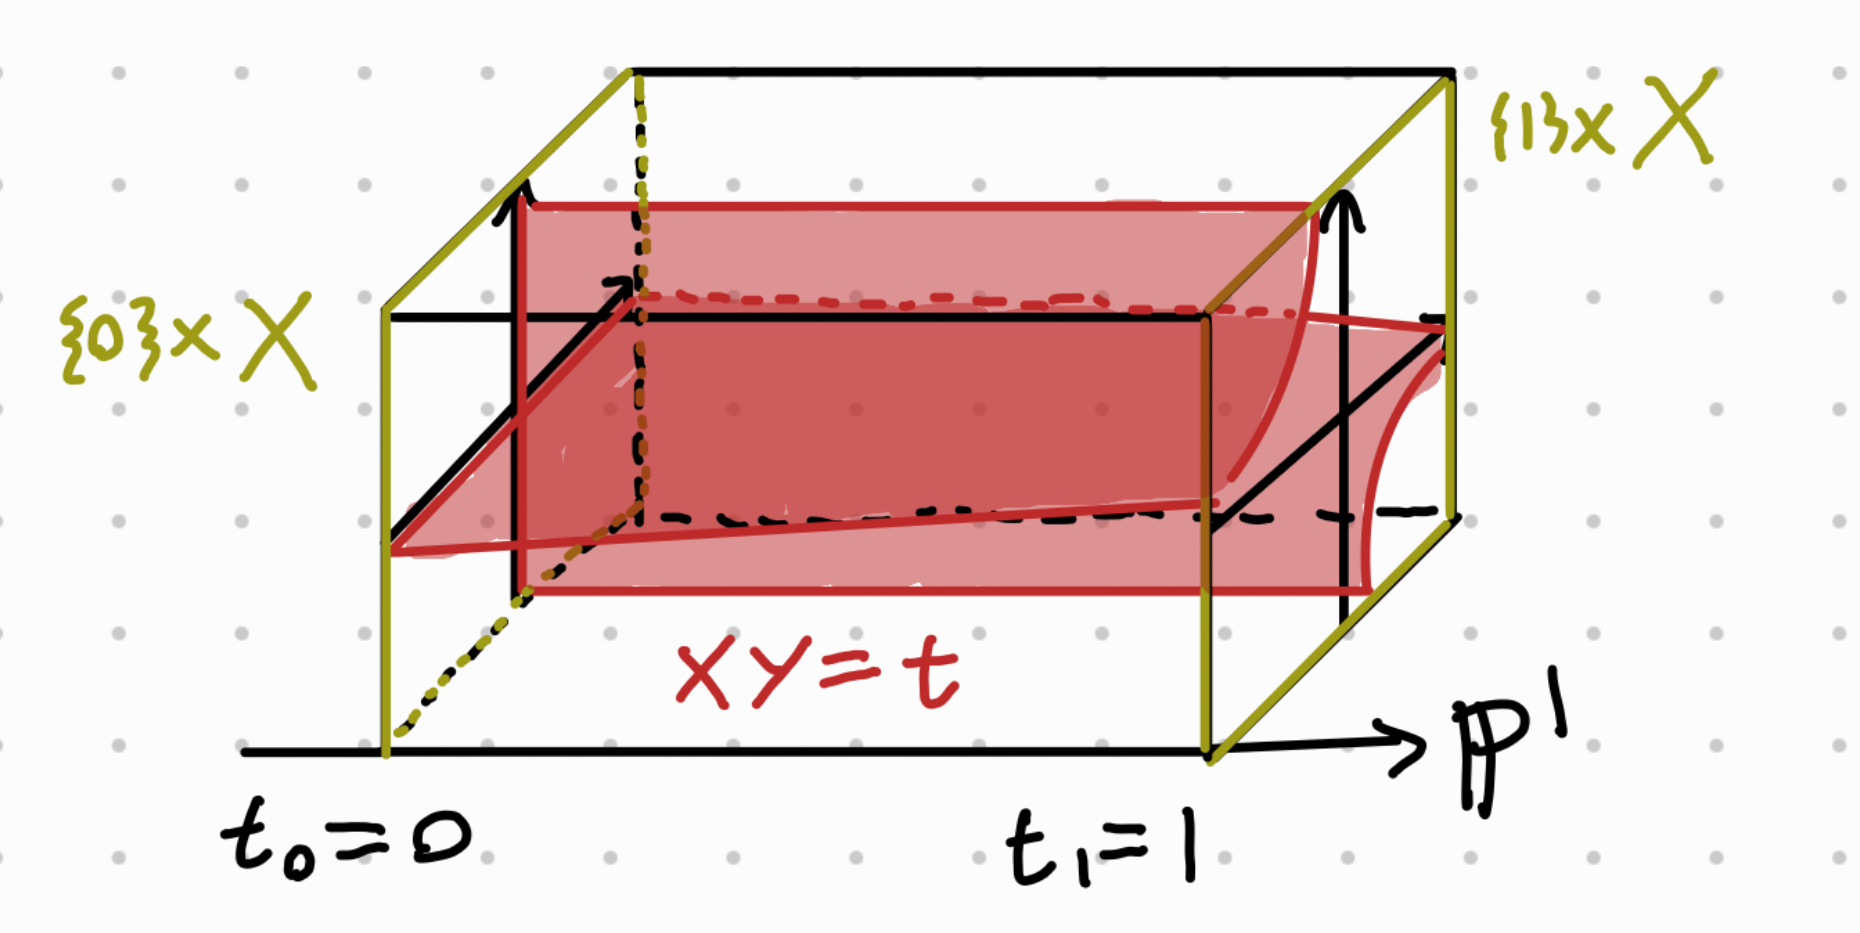
\includegraphics[width=9cm]{Images/rational-equivalence.png}
\end{figure}
\end{example}

\begin{remark}
It may be useful to think of rational equivalence as some type of homotopy equivalence. This would make the Chow ring something akin to the cohomology ring of the varieties. These analogies are beatiful and deep, but we shall not persue them further.
\end{remark}



\begin{example}
In $\A^2$ all points are rationally equivalent. To find the relation just multiply $\Pj^1$ with $\A^2$ and consider the line which connects the two points at different slices like in the picture
\begin{figure}[!htb]
	\centering
	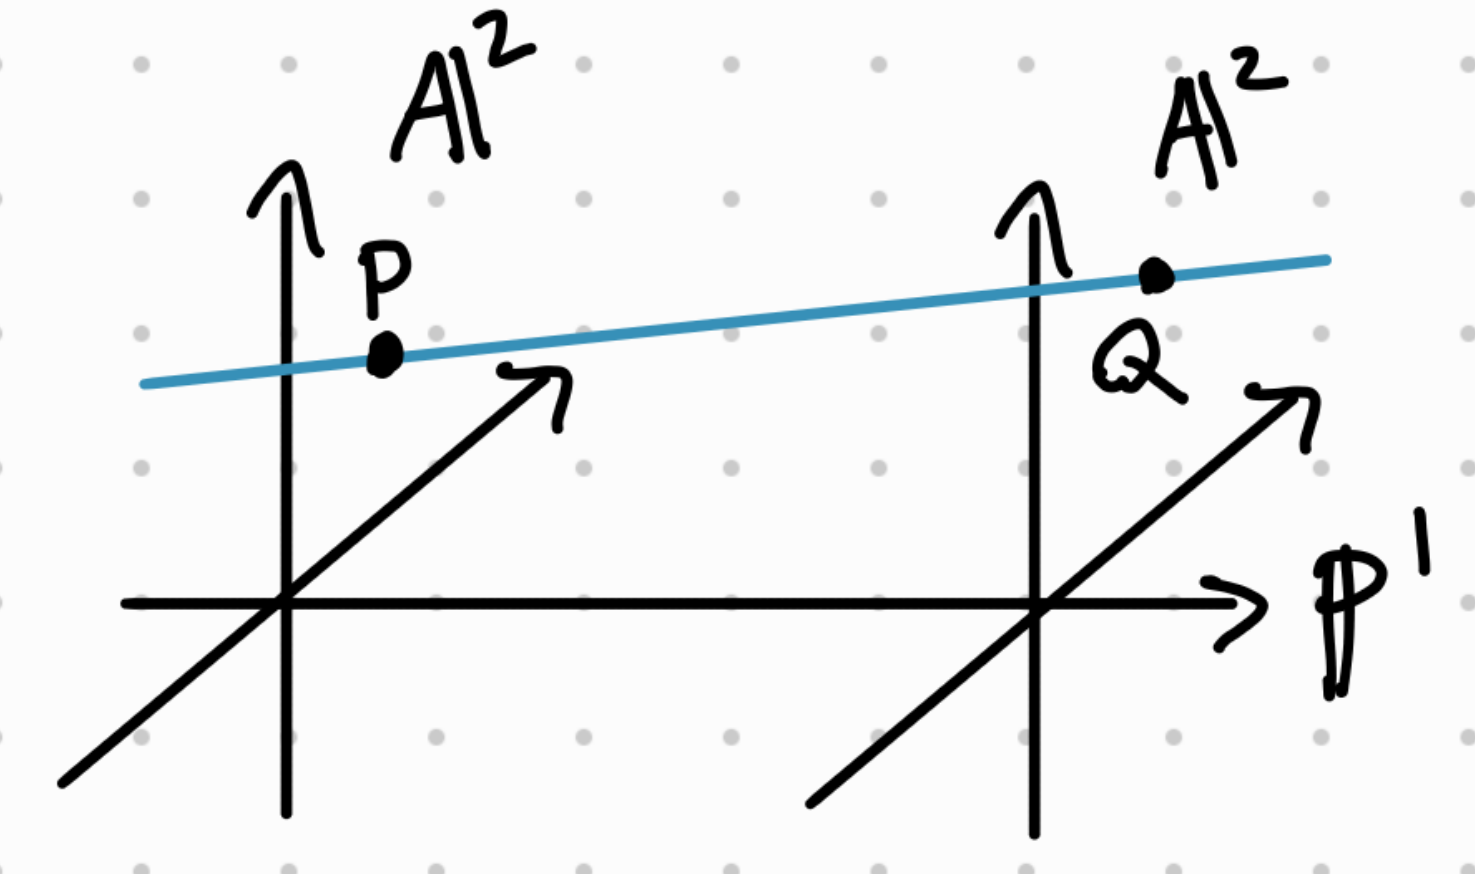
\includegraphics[width=6cm]{Images/points-in-A2-are-rationally-equivalent.png}
\end{figure}
\end{example}

\begin{example}
In $\A^2$, all lines passing through the origin are rationally equivalent.
Recall that $\GL_2$ acts on $\A^2$ and that $\GL_2\subseteq \A^4$. Moreover, the orbit of some line $L$ under the action of $\GL_2$ yiels all lines. This suggests a way to construct a rational equivalence between $[L]$ and $[gL]$ for $g\in \GL_2$.

The idea is to take the line $g(t)$ in $\A^4$ which connects $id\in \GL_2$ to $g\in \GL_2$ and then consider $\Phi$ to be the variety where each slice corresponds to $g(t)L$.
\end{example}


\subsection{Chow ring}
Now that we have our objects that we want to intersect, we want to count the ``number of intersections" somehow. 

If we think about this, we find a problem when trying to define what the intersection ought to be when tangencies are involved. For example, if we intersect a line with a circle we always get two intersection points except when the line is tangent to the circle, in which case the two intersection points \textit{collapse} to a single point. We want to count that as an intersection of multiplicity 2, not a single intersection.

\begin{figure}[!htb]
	\centering
	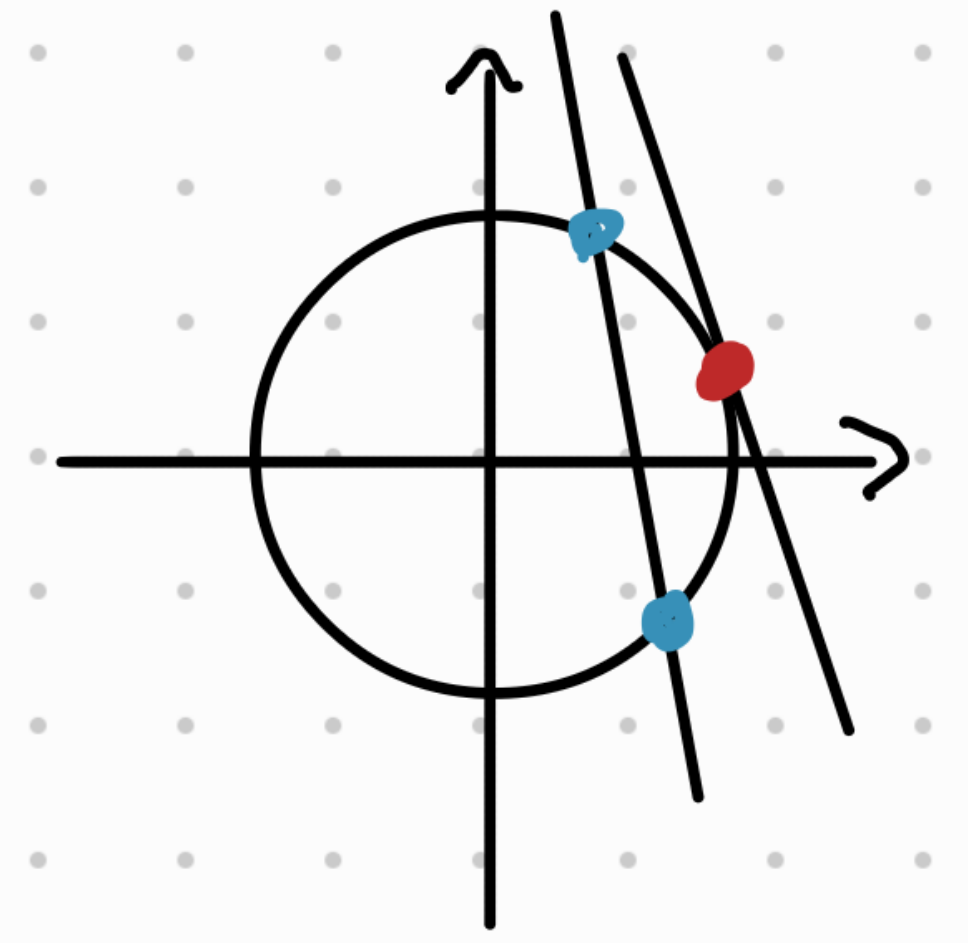
\includegraphics[width=4cm]{Images/tangent-moves-to-transverse.png}
\end{figure}

Let us define the ``well behaved" cases of intersection first:

\begin{definition}[]
Let $A,B$ be integral subvarieties of $X$. We say that $A$ and $B$ are \textbf{transverse} at $p\in A\cap B$ if $T_pA+T_pB=T_pX$, i.e. 
\[\codim T_p A+\codim T_p B=\codim(T_pA\cap T_p B).\]
We say that $A$ and $B$ are \textbf{generically transverse} if they are transverse at all generic points of the intersection.
\end{definition}

We now cite a lemma which tells us that we may reduce ``ill behaved" cases to ``well behaved" ones

\begin{lemma}[Moving lemma]
Let $X$ be a smooth quasi-projective variety, then the following holds:
\begin{itemize}
\item For all $\al,\beta\in CH(X)$ there exist $A,B\in Z(X)$ such that $\al=[A]$, $\beta=[B]$ and $A,B$ are generically transverse.
\item The class $[A\cap B]$ depends only on $[A]$ and $[B]$, not the representatives $A,B$.
\end{itemize}
\end{lemma}

With this lemma we can now put a product on $CH(X)$ which formalizes intersection, making it a ring.

\begin{theorem}
Let $X$ be smooth and quasi-projective, then there exists a unique product on $CH(X)$ such that for all $A,B$ subvarieties of $X$, if they are generically transverse then $[A]\cdot [B]=[A\cap B]$.

This makes $CH(X)$ into a graded (by codimension), associative, commutative and unital ring.
\end{theorem}

\begin{remark}
The identity of the Chow ring of $X$ is the \textbf{fundemental class}, i.e. $[X]$. This has degree (codimension) $0$ as we would expect. Intuitively, this corresponds to the simple fact that
\[A\subseteq X\implies A\cap X=A.\]
\end{remark}


\subsection{Non-triviality}

The first non-triviality result concerns codimention 0 cycles, that is, irreducible components of the ambient variety.
\begin{theorem}
If $X$ is irreducible and $\dim X=n$ then $CH_n(X)=CH^0(X)\cong \Z$ and it is generated by $[X]$.

If $X$ has irreducible components given by $X_1,\cdots, X_r$, then $[X_1],\cdots, [X_r]$ generate a free abelian subgroup of $CH(X)$ which is isomorphic to $\Z^r$.
\end{theorem}
\begin{proof}[Sketch]
If $\Phi\subseteq X\times \Pj^1$ gives some rational equivalence then $\Phi\subseteq X_i\times \Pj^1$ by irreducibility. So we may only consider the irreducible case.
If $\Phi\cap (\cpa{t_0}\times X)=X$ then $\Phi=X\times \Pj^1$, again by irreduciblity.
\end{proof}

\noindent
When considering codimension 1 we get back the theory of divisors as one would expect
\begin{proposition}
Suppose $X$ is irreducible of dimension $n$, then
\[CH_{n-1}(X)=CH^1(X)\cong \Pic(X)\]
and the correspondence is that the divisor $D=\sum n_i Y_i$ corresponds to $\sum n_i[Y_i]$.
\end{proposition}
\begin{proof}[Rough sketch]
The correspondence is clear at the level of $Z(X)$ and $\Div(X)$. What we need to see is that the two equivalence relations translate into each other.
If $f\in k(X)$ then we may take $\Phi=V(f(x)-t)$ to see that $[\cpa{f=0}]=[\cpa{f=\infty}]$, so $\mathrm{div}(f)$ does map to something in $\Rat(X)$.
To conclude we would need to show that $\Rat(X)$ is generated by the relations induced by principals divisors in this way.
\end{proof}


\section{Mayer-Vietoris and Excision}

Given the resemblance we noted before with cohomology rings, the following theorems seem rather natural (though we will not provide proofs):

\begin{theorem}[Mayer-Vietoris]
Let $X_1,X_2\subseteq X$ closed subvarieties, then we have an exact sequence
\[CH(X_1\cap X_2)\to CH(X_1)\oplus CH(X_2)\to CH(X_1\cup X_2)\to 0.\]
\end{theorem}


\begin{theorem}[Excision]
Let $Y\subseteq X$ be a closed subvariety, then we have an exact sequence
\[CH(Y)\to CH(X)\to CH(X\bs Y)\to 0\]
\end{theorem}

\begin{remark}
The exact sequence above may also be called \textit{the localization sequence}.
\end{remark}




\subsection{Issue with Chow rings of affine space}

Having now defined Chow rings, we want to compute some of them explicitly. We might attempt this first with affine space, but we start to run into some issues


\begin{example}
If we think about the Chow ring of spaces like $\A^2$ we start to run into some problems. For example, consider $[C]^2$ for $C$ some circle. To compute this intersection we may move a little one copy of the circle as in the picture
\begin{figure}[!htb]
	\centering
	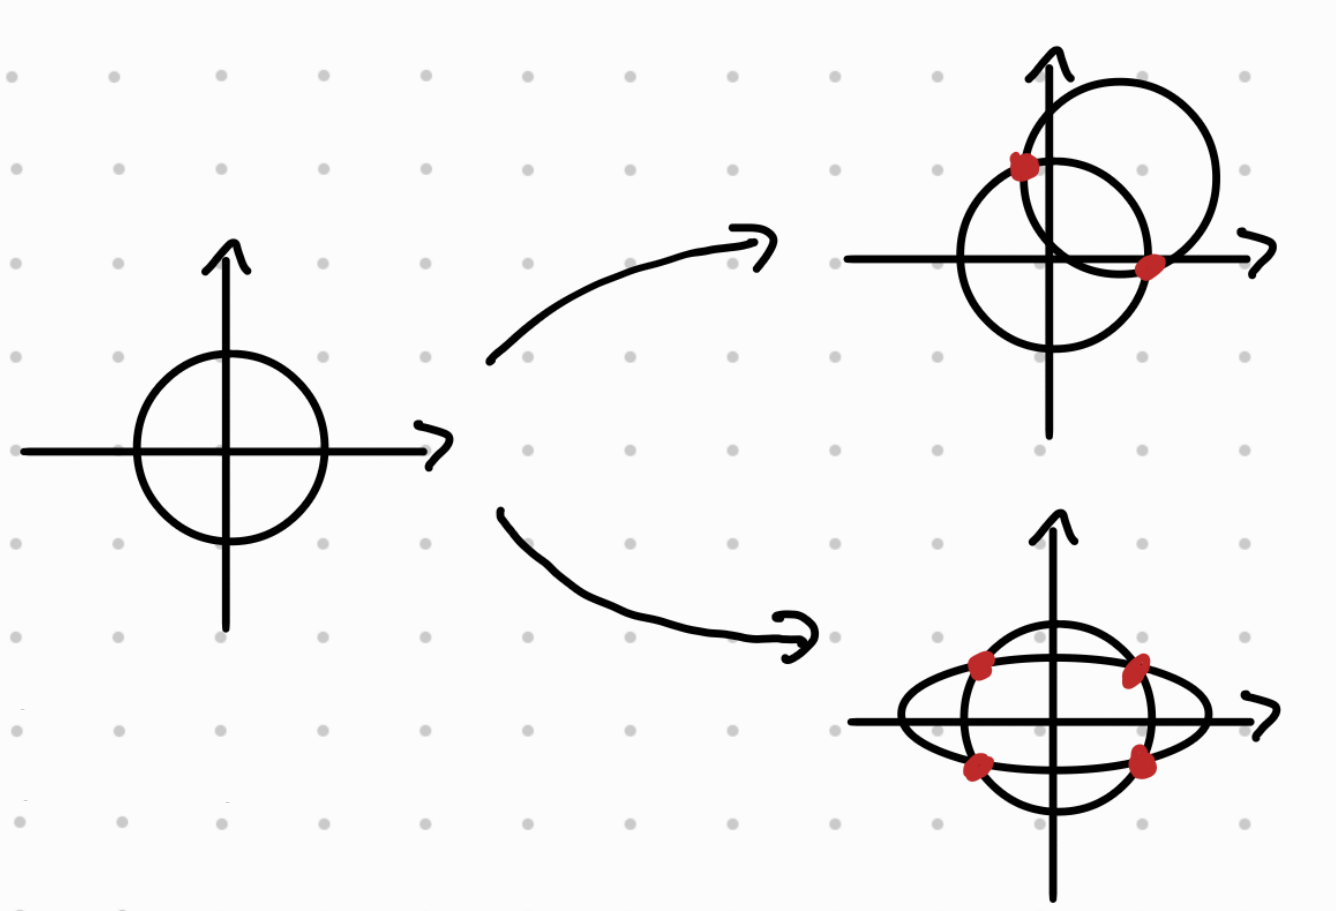
\includegraphics[width=8cm]{Images/circle-intersect-itself.png}
\end{figure}

The issue is that in the bottom case the four points of intersection are still in the affine plane, but in the top case they are at infinity, yielding some undesidered consequences which we will make more explicit in the next result.
\end{example}


\begin{proposition}
The Chow ring of affine space is $CH(\A^n)=\Z[\A^n]\cong \Z$, concentrated in degree 0.
\end{proposition}
\begin{proof}
Let $Y$ be any positive-codimension cycle and move it\footnote{translated copies of the same cycle are clearly rationally equivalent.} so that it does not pass through $0$.
We define\footnote{by $f(z/t)$ what we really mean is: if $t=x_1/x_0$ is the coordinate of $\Pj^1$, take $f$ and homogenize it with respect to $x_1$ to get $H_{x_1}(f)$. By the notation $f(z/t)$ we mean $(H_{x_1}(f)(x_0 z))/(x_1^{\deg f})$.}
\[\Phi=\cpa{(t,ty)\mid y\in Y,\ t\in \A^1}=V(\cpa{f(z/t)\mid f\in I(Y)})\subseteq \Pj^1\times \A^n.\]
Let us consider the slices of $\Phi$ at $t_0=1$ and $t_1=\infty$: 
\setlength{\leftmargini}{0cm}
\begin{itemize}
\item[$\boxed{t=1}$] The ideal is $I(Y)$ itself ($f(z/1)=f(z)$) and we get back $Y$.
\item[$\boxed{t=\infty}$] Since $Y$ does not go through $0$, there is some $f\in I(Y)$ such that $f(0)\neq 0$. If we take the slice at $\infty$ we get that $f(z/\infty)=f(0)\neq 0$ is in the ideal which defines $\Phi\cap \cpa{\infty}\times \A^n$, so the slice is $\emptyset$.
\end{itemize}
\setlength{\leftmargini}{0.5cm}
We have just shown that $\Phi$ defines an equivalence between $Y$ and $\emptyset$, meaning that all cycles in positive codimension are $0$ in the cohomology ring.
\end{proof}

\begin{corollary}
If $U\subseteq \A^n$ open, $CH(U)\cong \Z$ with generator $[U]$.
\end{corollary}
\begin{proof}[Idea]
Use excision.
\end{proof}


\begin{center}
The bottom line is that ``good intersection theory" requires some properness condition.
\end{center}


\section{Functoriality and proper push-forward}
Like all good constructions, if we build Chow rings for objects we want to have homomorphisms which are induced by maps between objects. Unfortunaltely this is rather tricky. The morphisms between schemes have to be proper to have a nice pushforward between the Chow rings. 

\begin{remark}
If $f:X\to Y$ is proper and $A\subseteq X$ subvariety then $f(A)^{red}\subseteq Y$ is a subvariety.
\end{remark}



\begin{theorem}
If $f:X\to Y$ proper, we can get $f_\ast:CH(X)\to CH(Y)$. On generators it behaves as follows
\[f_\ast[A]=\begin{cases}
0 &\text{if }\dim f(A)<\dim A\\
d[f(A)] &\text{if }\dim f(A)=\dim A\text{ and }d=\deg(A\to f(A))
\end{cases}\]
\end{theorem}

\begin{theorem}
$f_\ast$ defines a dimension-preserving morphism of the Chow-groups
\end{theorem}

\begin{figure}[!htb]
	\centering
	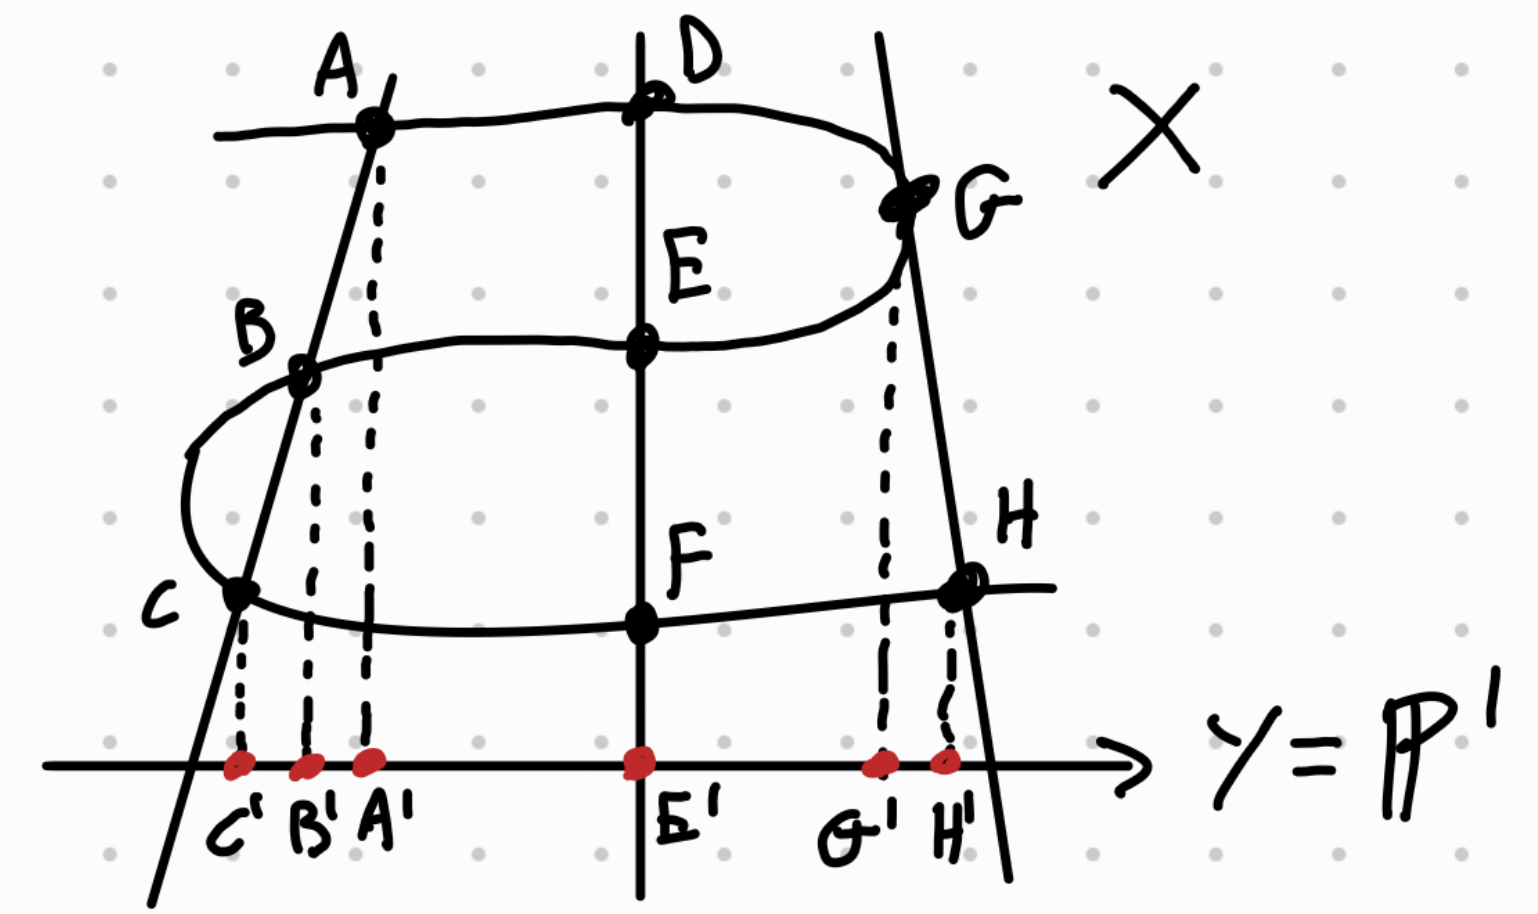
\includegraphics[width=7cm]{Images/degree-pushforward.png}
	\caption{The cycle $A+B+C\sim D+E+F\sim 2G+H$, gets mapped to $A'+B'+C'\sim 3E'\sim 2G'+H'$. In all cases multiplicities are preserved.}
\end{figure}


\begin{proposition}
If $X\to \Spec k$ is proper, then we have a unique map $\deg:CH(X)=CH(pt)\cong \Z$ which preserves dimension (so $[Y]\mapsto 0$ if $\dim Y>0$ and $[pt]\mapsto 1$).
\end{proposition}



\section{Projective space}
Since properness seems to play a big role in this theory, we compute the Chow ring of projective space.

\begin{definition}[]
Let $X\subseteq \Pj^n$ be an irreducible closed subvariety of dimension $k$. The \textbf{degree} of $X$ is the number of intersection points, counted with multiplicities, it has when intersected with $k$ hyperplanes in general position.
\end{definition}

\begin{remark}
The following is an equivalent, but perhaps more reassuring, definition of degree: let 
\[P(t)=\frac{h(t)}{(1-t)^k},\quad h(t)\in \Z[t],\ h(1)\neq 0\]
be the Poincar\'e-Hilbert series of $X\subseteq \Pj^n$, then the degree of $X$ is $h(1)$.
\end{remark}

\begin{definition}[]
Let $X$ be a scheme of finite type of $k$. We call a finite collection of irreducible locally closed subschemes $X_i$ an \textbf{affine stratification} if 
\begin{itemize}
\item each $X_i$ is isomorphic to some $\A^{k_i}$,
\item $X$ is the disjoint union of the $X_i$,
\item the closure of each $X_i$ us given by a union of some $X_j$.
\end{itemize}
\end{definition}

\begin{theorem}
We have that as graded rings
\[CH(\Pj^n)\cong \frac{\Z[t]}{(t^{n+1})}\]
where $t$ is the class of some linear hyperplane. Moreover, if $X\subseteq \Pj^n$ irreducible of codimension $k$ and degree $d$ then $[X]=dt^k$.
\end{theorem}
\begin{proof}[Sketch]
The proof consists of the following steps
\setlength{\leftmargini}{0cm}
\begin{itemize}
\item Consider the chain of inclusions
\[\cpa{pt}=\Pj^0\subseteq \Pj^1\subseteq\cdots\subseteq \Pj^n\]
given by fixing the last free coordinate to be $0$ to get from one term to the previous one. Consider the differences $U_i=\Pj^i\bs \Pj^{i-1}$, which are all isomorphic to affine space. It turns out that the $U_i$ form an {affine stratification} of $\Pj^n$.
\item Prove that $CH(\Pj^n)$ is generated by the classes of $[\ol{U_i}]$. The idea to prove the result for general affine stratifications. Proceed by induction on the number of strata. Let $U_0$ be a minimal strata and note that beacuse of that $\ol{U_0}=U_0$. By excision we have:
\[\Z=CH({U_0})=CH(\ol{U_0})\to CH(X)\to CH(X\bs \ol{U_0})\to 0\]
and the last bit is a scheme with affine stratification that has one less strata, therefore the Chow ring of the last term is generated by the $[\ol{U_i}]$ for $i\neq 0$ by inductive hypothesis. 
\item Intersecting $k$ hyperplanes gives a $(n-k)$-plane, so $t^k=[(n-k)\text{-plane}]$.
\item Let $M\subseteq \Pj^n$ be an $k$-plane, we have a surjective\footnote{$(n-k)$-plane $\cap$ $k$-plane $=[pt]$, generator of $CH^n(\Pj^n)$} map
% https://q.uiver.app/#q=WzAsMyxbMCwwLCJDSF5rKFxcUGpebikiXSxbMSwwLCJDSF5uKFxcUGpebikiXSxbMiwwLCJDSChwdCkiXSxbMCwxLCJcXGNkb3QgW01dIl0sWzEsMiwiPSIsMyx7InN0eWxlIjp7ImJvZHkiOnsibmFtZSI6Im5vbmUifSwiaGVhZCI6eyJuYW1lIjoibm9uZSJ9fX1dLFswLDIsIlxcZGVnIiwyLHsiY3VydmUiOjJ9XV0=
\[\begin{tikzcd}
	{CH^k(\Pj^n)} & {CH^n(\Pj^n)} & {CH(pt)}
	\arrow["{\cdot [M]}", from=1-1, to=1-2]
	\arrow["\deg"', curve={height=12pt}, from=1-1, to=1-3]
	\arrow["{=}"{marking, allow upside down}, draw=none, from=1-2, to=1-3]
\end{tikzcd}\]
and the full composition is the degree map, so this is also injective ($[X]$ is in the kernel when it has empty intersection with general $M$ and this cannot happen if $X$ has codimension $k$).
Thus $CH^k(\Pj^n)\cong \Z$ and this map is actually an isomorphism of abelian groups. Moreover, if $[X]\in CH^k(\Pj^n)$ then\footnote{by definition, the degree of an $(n-k)$-subvariety is the number of intersections with a general $k$-plane} 
\[[X][M]=\deg X [pt]=\deg X t^n=(\deg X t^{k})t^{n-k}=(\deg X t^{k})[M]\] 
and so $[X]=\deg Xt^k$.
\end{itemize}
\setlength{\leftmargini}{0.5cm}
\end{proof}

To get some practice with this ring we conclude with the following exercise

\begin{exercise}
In $\A^2$ draw three circles $C_1,\ C_2,\ C_3$. 
\begin{figure}[!htb]
	\centering
	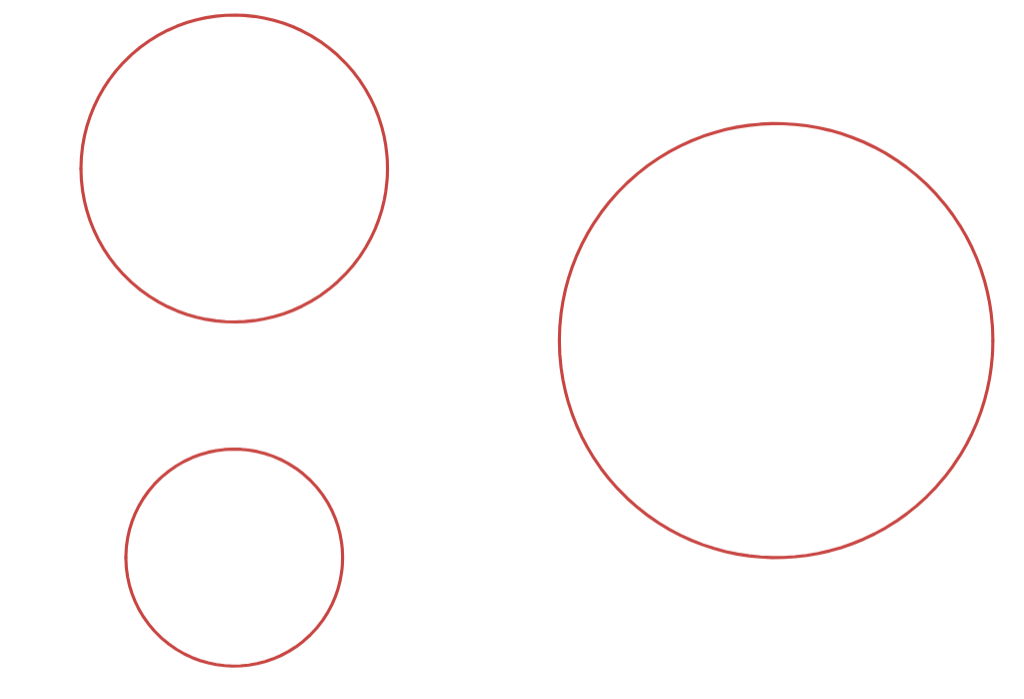
\includegraphics[width=4cm]{Images/Three-circles.png}
\end{figure}

How many circles can be drawn which are tangent to $C_1$, $C_2$ and $C_3$?
\end{exercise}
\begin{proof}[Solution]
A circle in the plane is given by an equation of the form $(x-A)^2+(y-B)^2=C$. If we homogenize we see that the two points at infinity $[1:\pm i:0]$ always lie on such a homogenized circle. We may therefore define a circle in $\Pj^2$ to be a conic which passes through these two points.

Recall that conics in $\Pj^2$ are parametrized by $\Pj^5$ by looking at the coefficients in their general equation
\[ax^2+bxy+cy^2+dxz+ezy+fz^2=0.\]
By imposing the fact that the circles should go through two distinct points we get that circles are parametrized by a $\Pj^3$. More precisely, they correspond to the intersection of the two hypersurfaces $a+bi-c=0$ and $a-bi-c=0$ in $\Pj^5$.


What does it mean for a circle to be tangent to another fixed circle $C$? Let $Z_C=\cpa{\text{circles tangent to $C$}}\subseteq\Pj^3$ and consider the pairs
\[\Phi=\cpa{(r,D)\mid r\in C,\ D \text{ circle tangent to $C$ at $r$}}.\]
We have two projections $\Phi\to C$ and $\Phi\to Z_C$. Note that the fibers of $\Phi\to C$ are isomorphic to $\Pj^1$: up to translation, suppose that $r=0$. If $D$ is some circle which is tangent to $C$ at $0$ then all circles which are tangent to $C$ at that same point are re-scaled versions of $D$. 

\begin{figure}[!htb]
	\centering
	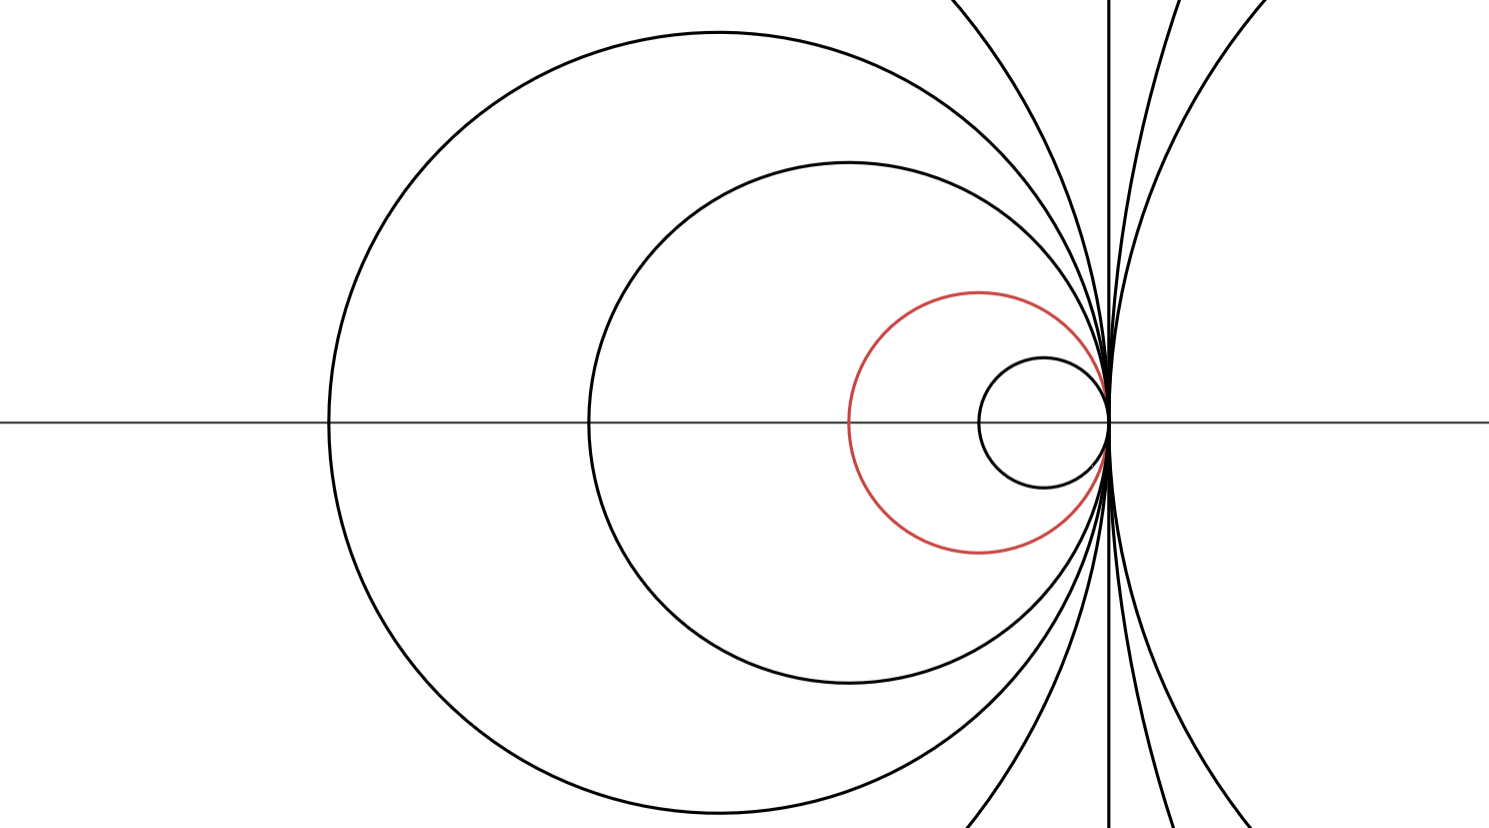
\includegraphics[width=7cm]{Images/pencil-of-tangent-circles.png}
\end{figure}

So $\Phi$ should be a surface of some kind (fiber bundle over a circle with fibers given by $\Pj^1$). This surface should have degree 2 because tangency between a circle $D:(x-a)^2+(y-b)^2=c$ and a fixed circle $C:(x-a_0)^2+(y-b_0)^2=c_0$ is checked by imposing that the following system of equations has a double solution 
\[\begin{cases}
	(x-a)^2+(y-b)^2=c\\
	(x-a_0)^2+(y-b_0)^2=c_0
\end{cases}\]
and the way we impose that is by setting the discriminant of a resulting quadratic equation to be 0. The fact that the degree should be two comes from the fact that the discriminant has degree two in the coefficients of the equation.

Moreover, $Z_C$ is birational to $\Phi$ (from a circle in $Z_C$ we can get the point of tangency it has with $C$).

So $Z_{C_1}\subseteq\Pj^3$ is a surface of degree 2. In the Chow group $CH(\Pj^3)$ we thus have $2t=[Z_{C_1}]$ and so
\[[Z_{C_1}\cap Z_{C_2}\cap Z_{C_3}]=[Z_{C_1}][Z_{C_2}][Z_{C_3}]=(2t)^3=8t^3.\]
$8t^3\in CH(\Pj^3)$ is the class of eight points, so \textit{8 is the number we were looking for\footnote{when the three circles are in general enough position}}.
\end{proof}



















\appendix
\bibliographystyle{alpha}
\bibliography{refs}

\end{document}
